\documentclass[aspectratio=169]{beamer}
% Shared preamble for ml/ slide decks.
% Each lecture .tex starts with:
%   \documentclass[aspectratio=169]{beamer}
%   % Shared preamble for ml/ slide decks.
% Each lecture .tex starts with:
%   \documentclass[aspectratio=169]{beamer}
%   % Shared preamble for ml/ slide decks.
% Each lecture .tex starts with:
%   \documentclass[aspectratio=169]{beamer}
%   \input{../preamble}
% Compile from inside the chapter folder so \input{../preamble} resolves.

\usetheme{default}
\usecolortheme{dove}

\setbeamertemplate{navigation symbols}{}
\setbeamertemplate{footline}{%
  \hfill{\large\insertframenumber\,/\,\inserttotalframenumber}\hspace{0.8em}\vspace{0.5em}%
}

% Project palette (existing, kept for backwards compatibility with deferred/*)
\definecolor{popblue}{RGB}{52, 101, 164}
\definecolor{sampred}{RGB}{204, 0, 0}
\definecolor{paramgreen}{RGB}{0, 140, 70}
\definecolor{warnred}{RGB}{180, 40, 40}
\definecolor{orange1}{RGB}{220, 120, 0}
\definecolor{violet1}{RGB}{120, 50, 160}
\definecolor{lightbg}{RGB}{245, 245, 250}

% Armenian flag palette (use these for any 3-color highlight; per CLAUDE.md).
% "Nice versions": slightly de-saturated from the official spec for slide use,
% so they don't burn out under projector colors. Originals kept as *_pure.
\definecolor{armred}{RGB}{200, 30, 40}      % nice red (official #D90012 muted)
\definecolor{armblue}{RGB}{30, 70, 160}     % nice blue (official #0033A0 muted)
\definecolor{armorange}{RGB}{230, 160, 30}  % nice orange (official #F2A800 muted)
\definecolor{armred_pure}{HTML}{D90012}     % official Armenian flag red
\definecolor{armblue_pure}{HTML}{0033A0}    % official Armenian flag blue
\definecolor{armorange_pure}{HTML}{F2A800}  % official Armenian flag orange

\setbeamercolor{frametitle}{fg=popblue}
\setbeamercolor{title}{fg=popblue}

\usepackage{pgfplots}
\usepackage{tikz}
\usetikzlibrary{shapes, arrows.meta, positioning, calc, decorations.pathreplacing, patterns, matrix}
\pgfplotsset{compat=1.18}
\usepackage{amsmath, amssymb, amsfonts}
\usepackage{bm}
\usepackage{dsfont}
\usepackage{array}
\usepackage{pifont}
\usepackage{colortbl}
\usepackage{fontenc}

% Callout boxes. Purely additive - existing decks are unaffected.
% Usage: \begin{tcolorbox}[colback=armblue!8, colframe=armblue, boxrule=0.6pt, arc=2pt,
%                          title=\textbf{Key idea}] ... \end{tcolorbox}
% Palette convention (ml/SLIDE_STYLE.md): armblue=key idea, armred=trap/warning,
% paramgreen=takeaway or "Next", armorange=watch-out.
\usepackage[most]{tcolorbox}

% Cleaner table rules (\toprule, \midrule, \bottomrule). Also purely additive.
\usepackage{booktabs}

% \cancel{...} for struck-through terms in derivations (added 2026-08-11 for the
% importance-sampling frame in ch11_rl, where the dynamics cancel). Purely additive.
\usepackage{cancel}

% Minimal ML notation macros (subset of slds-lmu latex-math/basic-ml.tex).
% Kept here so we don't have to inline-expand every \thetav, \xv, etc.
% when porting upstream slides.
\newcommand{\R}{\mathds{R}}
\newcommand{\N}{\mathds{N}}
\newcommand{\E}{\mathds{E}}
\newcommand{\Xspace}{\mathcal{X}}
\newcommand{\Yspace}{\mathcal{Y}}
\newcommand{\Hspace}{\mathcal{H}}
\newcommand{\D}{\mathcal{D}}
\newcommand{\Dtrain}{\mathcal{D}_{\text{train}}}
\newcommand{\Dtest}{\mathcal{D}_{\text{test}}}
\newcommand{\xv}{\mathbf{x}}
\newcommand{\yv}{\mathbf{y}}
\newcommand{\Xmat}{\mathbf{X}}
\newcommand{\id}{\mathbf{I}}
\newcommand{\thetav}{\bm{\theta}}
\newcommand{\thetah}{\hat{\bm{\theta}}}
\newcommand{\lamv}{\bm{\lambda}}
\newcommand{\fx}{f(\xv)}
\newcommand{\fxt}{f(\xv \,|\, \bm{\theta})}
\newcommand{\fxi}{f\!\left(\xv^{(i)}\right)}
\newcommand{\fh}{\hat{f}}
\newcommand{\fxh}{\hat{f}(\xv)}
\newcommand{\yh}{\hat{y}}
\newcommand{\yih}{\hat{y}^{(i)}}
% \xi clashes with the Greek letter \xi; write \xv^{(i)} inline instead.
\newcommand{\yi}[1][i]{y^{(#1)}}
\newcommand{\xyi}[1][i]{\left(\xv^{(#1)},\, y^{(#1)}\right)}
\newcommand{\thx}{\bm{\theta}^\top \xv}
\newcommand{\sumin}{\sum_{i=1}^{n}}
\newcommand{\sumjp}{\sum_{j=1}^{p}}
\newcommand{\Lxy}{L\!\left(y, \fx\right)}
\newcommand{\Lxyi}{L\!\left(\yi, \fxi\right)}
\newcommand{\risk}{\mathcal{R}}
\newcommand{\riske}{\mathcal{R}_{\text{emp}}}
\newcommand{\risket}{\mathcal{R}_{\text{emp}}(\bm{\theta})}
\newcommand{\riskt}{\mathcal{R}(\bm{\theta})}
\newcommand{\riskr}{\mathcal{R}_{\text{reg}}}
\newcommand{\argmin}{\mathop{\mathrm{arg\,min}}}
\newcommand{\argmax}{\mathop{\mathrm{arg\,max}}}
\newcommand{\eps}{\varepsilon}

% Compile from inside the chapter folder so % Shared preamble for ml/ slide decks.
% Each lecture .tex starts with:
%   \documentclass[aspectratio=169]{beamer}
%   \input{../preamble}
% Compile from inside the chapter folder so \input{../preamble} resolves.

\usetheme{default}
\usecolortheme{dove}

\setbeamertemplate{navigation symbols}{}
\setbeamertemplate{footline}{%
  \hfill{\large\insertframenumber\,/\,\inserttotalframenumber}\hspace{0.8em}\vspace{0.5em}%
}

% Project palette (existing, kept for backwards compatibility with deferred/*)
\definecolor{popblue}{RGB}{52, 101, 164}
\definecolor{sampred}{RGB}{204, 0, 0}
\definecolor{paramgreen}{RGB}{0, 140, 70}
\definecolor{warnred}{RGB}{180, 40, 40}
\definecolor{orange1}{RGB}{220, 120, 0}
\definecolor{violet1}{RGB}{120, 50, 160}
\definecolor{lightbg}{RGB}{245, 245, 250}

% Armenian flag palette (use these for any 3-color highlight; per CLAUDE.md).
% "Nice versions": slightly de-saturated from the official spec for slide use,
% so they don't burn out under projector colors. Originals kept as *_pure.
\definecolor{armred}{RGB}{200, 30, 40}      % nice red (official #D90012 muted)
\definecolor{armblue}{RGB}{30, 70, 160}     % nice blue (official #0033A0 muted)
\definecolor{armorange}{RGB}{230, 160, 30}  % nice orange (official #F2A800 muted)
\definecolor{armred_pure}{HTML}{D90012}     % official Armenian flag red
\definecolor{armblue_pure}{HTML}{0033A0}    % official Armenian flag blue
\definecolor{armorange_pure}{HTML}{F2A800}  % official Armenian flag orange

\setbeamercolor{frametitle}{fg=popblue}
\setbeamercolor{title}{fg=popblue}

\usepackage{pgfplots}
\usepackage{tikz}
\usetikzlibrary{shapes, arrows.meta, positioning, calc, decorations.pathreplacing, patterns, matrix}
\pgfplotsset{compat=1.18}
\usepackage{amsmath, amssymb, amsfonts}
\usepackage{bm}
\usepackage{dsfont}
\usepackage{array}
\usepackage{pifont}
\usepackage{colortbl}
\usepackage{fontenc}

% Callout boxes. Purely additive - existing decks are unaffected.
% Usage: \begin{tcolorbox}[colback=armblue!8, colframe=armblue, boxrule=0.6pt, arc=2pt,
%                          title=\textbf{Key idea}] ... \end{tcolorbox}
% Palette convention (ml/SLIDE_STYLE.md): armblue=key idea, armred=trap/warning,
% paramgreen=takeaway or "Next", armorange=watch-out.
\usepackage[most]{tcolorbox}

% Cleaner table rules (\toprule, \midrule, \bottomrule). Also purely additive.
\usepackage{booktabs}

% \cancel{...} for struck-through terms in derivations (added 2026-08-11 for the
% importance-sampling frame in ch11_rl, where the dynamics cancel). Purely additive.
\usepackage{cancel}

% Minimal ML notation macros (subset of slds-lmu latex-math/basic-ml.tex).
% Kept here so we don't have to inline-expand every \thetav, \xv, etc.
% when porting upstream slides.
\newcommand{\R}{\mathds{R}}
\newcommand{\N}{\mathds{N}}
\newcommand{\E}{\mathds{E}}
\newcommand{\Xspace}{\mathcal{X}}
\newcommand{\Yspace}{\mathcal{Y}}
\newcommand{\Hspace}{\mathcal{H}}
\newcommand{\D}{\mathcal{D}}
\newcommand{\Dtrain}{\mathcal{D}_{\text{train}}}
\newcommand{\Dtest}{\mathcal{D}_{\text{test}}}
\newcommand{\xv}{\mathbf{x}}
\newcommand{\yv}{\mathbf{y}}
\newcommand{\Xmat}{\mathbf{X}}
\newcommand{\id}{\mathbf{I}}
\newcommand{\thetav}{\bm{\theta}}
\newcommand{\thetah}{\hat{\bm{\theta}}}
\newcommand{\lamv}{\bm{\lambda}}
\newcommand{\fx}{f(\xv)}
\newcommand{\fxt}{f(\xv \,|\, \bm{\theta})}
\newcommand{\fxi}{f\!\left(\xv^{(i)}\right)}
\newcommand{\fh}{\hat{f}}
\newcommand{\fxh}{\hat{f}(\xv)}
\newcommand{\yh}{\hat{y}}
\newcommand{\yih}{\hat{y}^{(i)}}
% \xi clashes with the Greek letter \xi; write \xv^{(i)} inline instead.
\newcommand{\yi}[1][i]{y^{(#1)}}
\newcommand{\xyi}[1][i]{\left(\xv^{(#1)},\, y^{(#1)}\right)}
\newcommand{\thx}{\bm{\theta}^\top \xv}
\newcommand{\sumin}{\sum_{i=1}^{n}}
\newcommand{\sumjp}{\sum_{j=1}^{p}}
\newcommand{\Lxy}{L\!\left(y, \fx\right)}
\newcommand{\Lxyi}{L\!\left(\yi, \fxi\right)}
\newcommand{\risk}{\mathcal{R}}
\newcommand{\riske}{\mathcal{R}_{\text{emp}}}
\newcommand{\risket}{\mathcal{R}_{\text{emp}}(\bm{\theta})}
\newcommand{\riskt}{\mathcal{R}(\bm{\theta})}
\newcommand{\riskr}{\mathcal{R}_{\text{reg}}}
\newcommand{\argmin}{\mathop{\mathrm{arg\,min}}}
\newcommand{\argmax}{\mathop{\mathrm{arg\,max}}}
\newcommand{\eps}{\varepsilon}
 resolves.

\usetheme{default}
\usecolortheme{dove}

\setbeamertemplate{navigation symbols}{}
\setbeamertemplate{footline}{%
  \hfill{\large\insertframenumber\,/\,\inserttotalframenumber}\hspace{0.8em}\vspace{0.5em}%
}

% Project palette (existing, kept for backwards compatibility with deferred/*)
\definecolor{popblue}{RGB}{52, 101, 164}
\definecolor{sampred}{RGB}{204, 0, 0}
\definecolor{paramgreen}{RGB}{0, 140, 70}
\definecolor{warnred}{RGB}{180, 40, 40}
\definecolor{orange1}{RGB}{220, 120, 0}
\definecolor{violet1}{RGB}{120, 50, 160}
\definecolor{lightbg}{RGB}{245, 245, 250}

% Armenian flag palette (use these for any 3-color highlight; per CLAUDE.md).
% "Nice versions": slightly de-saturated from the official spec for slide use,
% so they don't burn out under projector colors. Originals kept as *_pure.
\definecolor{armred}{RGB}{200, 30, 40}      % nice red (official #D90012 muted)
\definecolor{armblue}{RGB}{30, 70, 160}     % nice blue (official #0033A0 muted)
\definecolor{armorange}{RGB}{230, 160, 30}  % nice orange (official #F2A800 muted)
\definecolor{armred_pure}{HTML}{D90012}     % official Armenian flag red
\definecolor{armblue_pure}{HTML}{0033A0}    % official Armenian flag blue
\definecolor{armorange_pure}{HTML}{F2A800}  % official Armenian flag orange

\setbeamercolor{frametitle}{fg=popblue}
\setbeamercolor{title}{fg=popblue}

\usepackage{pgfplots}
\usepackage{tikz}
\usetikzlibrary{shapes, arrows.meta, positioning, calc, decorations.pathreplacing, patterns, matrix}
\pgfplotsset{compat=1.18}
\usepackage{amsmath, amssymb, amsfonts}
\usepackage{bm}
\usepackage{dsfont}
\usepackage{array}
\usepackage{pifont}
\usepackage{colortbl}
\usepackage{fontenc}

% Callout boxes. Purely additive - existing decks are unaffected.
% Usage: \begin{tcolorbox}[colback=armblue!8, colframe=armblue, boxrule=0.6pt, arc=2pt,
%                          title=\textbf{Key idea}] ... \end{tcolorbox}
% Palette convention (ml/SLIDE_STYLE.md): armblue=key idea, armred=trap/warning,
% paramgreen=takeaway or "Next", armorange=watch-out.
\usepackage[most]{tcolorbox}

% Cleaner table rules (\toprule, \midrule, \bottomrule). Also purely additive.
\usepackage{booktabs}

% \cancel{...} for struck-through terms in derivations (added 2026-08-11 for the
% importance-sampling frame in ch11_rl, where the dynamics cancel). Purely additive.
\usepackage{cancel}

% Minimal ML notation macros (subset of slds-lmu latex-math/basic-ml.tex).
% Kept here so we don't have to inline-expand every \thetav, \xv, etc.
% when porting upstream slides.
\newcommand{\R}{\mathds{R}}
\newcommand{\N}{\mathds{N}}
\newcommand{\E}{\mathds{E}}
\newcommand{\Xspace}{\mathcal{X}}
\newcommand{\Yspace}{\mathcal{Y}}
\newcommand{\Hspace}{\mathcal{H}}
\newcommand{\D}{\mathcal{D}}
\newcommand{\Dtrain}{\mathcal{D}_{\text{train}}}
\newcommand{\Dtest}{\mathcal{D}_{\text{test}}}
\newcommand{\xv}{\mathbf{x}}
\newcommand{\yv}{\mathbf{y}}
\newcommand{\Xmat}{\mathbf{X}}
\newcommand{\id}{\mathbf{I}}
\newcommand{\thetav}{\bm{\theta}}
\newcommand{\thetah}{\hat{\bm{\theta}}}
\newcommand{\lamv}{\bm{\lambda}}
\newcommand{\fx}{f(\xv)}
\newcommand{\fxt}{f(\xv \,|\, \bm{\theta})}
\newcommand{\fxi}{f\!\left(\xv^{(i)}\right)}
\newcommand{\fh}{\hat{f}}
\newcommand{\fxh}{\hat{f}(\xv)}
\newcommand{\yh}{\hat{y}}
\newcommand{\yih}{\hat{y}^{(i)}}
% \xi clashes with the Greek letter \xi; write \xv^{(i)} inline instead.
\newcommand{\yi}[1][i]{y^{(#1)}}
\newcommand{\xyi}[1][i]{\left(\xv^{(#1)},\, y^{(#1)}\right)}
\newcommand{\thx}{\bm{\theta}^\top \xv}
\newcommand{\sumin}{\sum_{i=1}^{n}}
\newcommand{\sumjp}{\sum_{j=1}^{p}}
\newcommand{\Lxy}{L\!\left(y, \fx\right)}
\newcommand{\Lxyi}{L\!\left(\yi, \fxi\right)}
\newcommand{\risk}{\mathcal{R}}
\newcommand{\riske}{\mathcal{R}_{\text{emp}}}
\newcommand{\risket}{\mathcal{R}_{\text{emp}}(\bm{\theta})}
\newcommand{\riskt}{\mathcal{R}(\bm{\theta})}
\newcommand{\riskr}{\mathcal{R}_{\text{reg}}}
\newcommand{\argmin}{\mathop{\mathrm{arg\,min}}}
\newcommand{\argmax}{\mathop{\mathrm{arg\,max}}}
\newcommand{\eps}{\varepsilon}

% Compile from inside the chapter folder so % Shared preamble for ml/ slide decks.
% Each lecture .tex starts with:
%   \documentclass[aspectratio=169]{beamer}
%   % Shared preamble for ml/ slide decks.
% Each lecture .tex starts with:
%   \documentclass[aspectratio=169]{beamer}
%   \input{../preamble}
% Compile from inside the chapter folder so \input{../preamble} resolves.

\usetheme{default}
\usecolortheme{dove}

\setbeamertemplate{navigation symbols}{}
\setbeamertemplate{footline}{%
  \hfill{\large\insertframenumber\,/\,\inserttotalframenumber}\hspace{0.8em}\vspace{0.5em}%
}

% Project palette (existing, kept for backwards compatibility with deferred/*)
\definecolor{popblue}{RGB}{52, 101, 164}
\definecolor{sampred}{RGB}{204, 0, 0}
\definecolor{paramgreen}{RGB}{0, 140, 70}
\definecolor{warnred}{RGB}{180, 40, 40}
\definecolor{orange1}{RGB}{220, 120, 0}
\definecolor{violet1}{RGB}{120, 50, 160}
\definecolor{lightbg}{RGB}{245, 245, 250}

% Armenian flag palette (use these for any 3-color highlight; per CLAUDE.md).
% "Nice versions": slightly de-saturated from the official spec for slide use,
% so they don't burn out under projector colors. Originals kept as *_pure.
\definecolor{armred}{RGB}{200, 30, 40}      % nice red (official #D90012 muted)
\definecolor{armblue}{RGB}{30, 70, 160}     % nice blue (official #0033A0 muted)
\definecolor{armorange}{RGB}{230, 160, 30}  % nice orange (official #F2A800 muted)
\definecolor{armred_pure}{HTML}{D90012}     % official Armenian flag red
\definecolor{armblue_pure}{HTML}{0033A0}    % official Armenian flag blue
\definecolor{armorange_pure}{HTML}{F2A800}  % official Armenian flag orange

\setbeamercolor{frametitle}{fg=popblue}
\setbeamercolor{title}{fg=popblue}

\usepackage{pgfplots}
\usepackage{tikz}
\usetikzlibrary{shapes, arrows.meta, positioning, calc, decorations.pathreplacing, patterns, matrix}
\pgfplotsset{compat=1.18}
\usepackage{amsmath, amssymb, amsfonts}
\usepackage{bm}
\usepackage{dsfont}
\usepackage{array}
\usepackage{pifont}
\usepackage{colortbl}
\usepackage{fontenc}

% Callout boxes. Purely additive - existing decks are unaffected.
% Usage: \begin{tcolorbox}[colback=armblue!8, colframe=armblue, boxrule=0.6pt, arc=2pt,
%                          title=\textbf{Key idea}] ... \end{tcolorbox}
% Palette convention (ml/SLIDE_STYLE.md): armblue=key idea, armred=trap/warning,
% paramgreen=takeaway or "Next", armorange=watch-out.
\usepackage[most]{tcolorbox}

% Cleaner table rules (\toprule, \midrule, \bottomrule). Also purely additive.
\usepackage{booktabs}

% \cancel{...} for struck-through terms in derivations (added 2026-08-11 for the
% importance-sampling frame in ch11_rl, where the dynamics cancel). Purely additive.
\usepackage{cancel}

% Minimal ML notation macros (subset of slds-lmu latex-math/basic-ml.tex).
% Kept here so we don't have to inline-expand every \thetav, \xv, etc.
% when porting upstream slides.
\newcommand{\R}{\mathds{R}}
\newcommand{\N}{\mathds{N}}
\newcommand{\E}{\mathds{E}}
\newcommand{\Xspace}{\mathcal{X}}
\newcommand{\Yspace}{\mathcal{Y}}
\newcommand{\Hspace}{\mathcal{H}}
\newcommand{\D}{\mathcal{D}}
\newcommand{\Dtrain}{\mathcal{D}_{\text{train}}}
\newcommand{\Dtest}{\mathcal{D}_{\text{test}}}
\newcommand{\xv}{\mathbf{x}}
\newcommand{\yv}{\mathbf{y}}
\newcommand{\Xmat}{\mathbf{X}}
\newcommand{\id}{\mathbf{I}}
\newcommand{\thetav}{\bm{\theta}}
\newcommand{\thetah}{\hat{\bm{\theta}}}
\newcommand{\lamv}{\bm{\lambda}}
\newcommand{\fx}{f(\xv)}
\newcommand{\fxt}{f(\xv \,|\, \bm{\theta})}
\newcommand{\fxi}{f\!\left(\xv^{(i)}\right)}
\newcommand{\fh}{\hat{f}}
\newcommand{\fxh}{\hat{f}(\xv)}
\newcommand{\yh}{\hat{y}}
\newcommand{\yih}{\hat{y}^{(i)}}
% \xi clashes with the Greek letter \xi; write \xv^{(i)} inline instead.
\newcommand{\yi}[1][i]{y^{(#1)}}
\newcommand{\xyi}[1][i]{\left(\xv^{(#1)},\, y^{(#1)}\right)}
\newcommand{\thx}{\bm{\theta}^\top \xv}
\newcommand{\sumin}{\sum_{i=1}^{n}}
\newcommand{\sumjp}{\sum_{j=1}^{p}}
\newcommand{\Lxy}{L\!\left(y, \fx\right)}
\newcommand{\Lxyi}{L\!\left(\yi, \fxi\right)}
\newcommand{\risk}{\mathcal{R}}
\newcommand{\riske}{\mathcal{R}_{\text{emp}}}
\newcommand{\risket}{\mathcal{R}_{\text{emp}}(\bm{\theta})}
\newcommand{\riskt}{\mathcal{R}(\bm{\theta})}
\newcommand{\riskr}{\mathcal{R}_{\text{reg}}}
\newcommand{\argmin}{\mathop{\mathrm{arg\,min}}}
\newcommand{\argmax}{\mathop{\mathrm{arg\,max}}}
\newcommand{\eps}{\varepsilon}

% Compile from inside the chapter folder so % Shared preamble for ml/ slide decks.
% Each lecture .tex starts with:
%   \documentclass[aspectratio=169]{beamer}
%   \input{../preamble}
% Compile from inside the chapter folder so \input{../preamble} resolves.

\usetheme{default}
\usecolortheme{dove}

\setbeamertemplate{navigation symbols}{}
\setbeamertemplate{footline}{%
  \hfill{\large\insertframenumber\,/\,\inserttotalframenumber}\hspace{0.8em}\vspace{0.5em}%
}

% Project palette (existing, kept for backwards compatibility with deferred/*)
\definecolor{popblue}{RGB}{52, 101, 164}
\definecolor{sampred}{RGB}{204, 0, 0}
\definecolor{paramgreen}{RGB}{0, 140, 70}
\definecolor{warnred}{RGB}{180, 40, 40}
\definecolor{orange1}{RGB}{220, 120, 0}
\definecolor{violet1}{RGB}{120, 50, 160}
\definecolor{lightbg}{RGB}{245, 245, 250}

% Armenian flag palette (use these for any 3-color highlight; per CLAUDE.md).
% "Nice versions": slightly de-saturated from the official spec for slide use,
% so they don't burn out under projector colors. Originals kept as *_pure.
\definecolor{armred}{RGB}{200, 30, 40}      % nice red (official #D90012 muted)
\definecolor{armblue}{RGB}{30, 70, 160}     % nice blue (official #0033A0 muted)
\definecolor{armorange}{RGB}{230, 160, 30}  % nice orange (official #F2A800 muted)
\definecolor{armred_pure}{HTML}{D90012}     % official Armenian flag red
\definecolor{armblue_pure}{HTML}{0033A0}    % official Armenian flag blue
\definecolor{armorange_pure}{HTML}{F2A800}  % official Armenian flag orange

\setbeamercolor{frametitle}{fg=popblue}
\setbeamercolor{title}{fg=popblue}

\usepackage{pgfplots}
\usepackage{tikz}
\usetikzlibrary{shapes, arrows.meta, positioning, calc, decorations.pathreplacing, patterns, matrix}
\pgfplotsset{compat=1.18}
\usepackage{amsmath, amssymb, amsfonts}
\usepackage{bm}
\usepackage{dsfont}
\usepackage{array}
\usepackage{pifont}
\usepackage{colortbl}
\usepackage{fontenc}

% Callout boxes. Purely additive - existing decks are unaffected.
% Usage: \begin{tcolorbox}[colback=armblue!8, colframe=armblue, boxrule=0.6pt, arc=2pt,
%                          title=\textbf{Key idea}] ... \end{tcolorbox}
% Palette convention (ml/SLIDE_STYLE.md): armblue=key idea, armred=trap/warning,
% paramgreen=takeaway or "Next", armorange=watch-out.
\usepackage[most]{tcolorbox}

% Cleaner table rules (\toprule, \midrule, \bottomrule). Also purely additive.
\usepackage{booktabs}

% \cancel{...} for struck-through terms in derivations (added 2026-08-11 for the
% importance-sampling frame in ch11_rl, where the dynamics cancel). Purely additive.
\usepackage{cancel}

% Minimal ML notation macros (subset of slds-lmu latex-math/basic-ml.tex).
% Kept here so we don't have to inline-expand every \thetav, \xv, etc.
% when porting upstream slides.
\newcommand{\R}{\mathds{R}}
\newcommand{\N}{\mathds{N}}
\newcommand{\E}{\mathds{E}}
\newcommand{\Xspace}{\mathcal{X}}
\newcommand{\Yspace}{\mathcal{Y}}
\newcommand{\Hspace}{\mathcal{H}}
\newcommand{\D}{\mathcal{D}}
\newcommand{\Dtrain}{\mathcal{D}_{\text{train}}}
\newcommand{\Dtest}{\mathcal{D}_{\text{test}}}
\newcommand{\xv}{\mathbf{x}}
\newcommand{\yv}{\mathbf{y}}
\newcommand{\Xmat}{\mathbf{X}}
\newcommand{\id}{\mathbf{I}}
\newcommand{\thetav}{\bm{\theta}}
\newcommand{\thetah}{\hat{\bm{\theta}}}
\newcommand{\lamv}{\bm{\lambda}}
\newcommand{\fx}{f(\xv)}
\newcommand{\fxt}{f(\xv \,|\, \bm{\theta})}
\newcommand{\fxi}{f\!\left(\xv^{(i)}\right)}
\newcommand{\fh}{\hat{f}}
\newcommand{\fxh}{\hat{f}(\xv)}
\newcommand{\yh}{\hat{y}}
\newcommand{\yih}{\hat{y}^{(i)}}
% \xi clashes with the Greek letter \xi; write \xv^{(i)} inline instead.
\newcommand{\yi}[1][i]{y^{(#1)}}
\newcommand{\xyi}[1][i]{\left(\xv^{(#1)},\, y^{(#1)}\right)}
\newcommand{\thx}{\bm{\theta}^\top \xv}
\newcommand{\sumin}{\sum_{i=1}^{n}}
\newcommand{\sumjp}{\sum_{j=1}^{p}}
\newcommand{\Lxy}{L\!\left(y, \fx\right)}
\newcommand{\Lxyi}{L\!\left(\yi, \fxi\right)}
\newcommand{\risk}{\mathcal{R}}
\newcommand{\riske}{\mathcal{R}_{\text{emp}}}
\newcommand{\risket}{\mathcal{R}_{\text{emp}}(\bm{\theta})}
\newcommand{\riskt}{\mathcal{R}(\bm{\theta})}
\newcommand{\riskr}{\mathcal{R}_{\text{reg}}}
\newcommand{\argmin}{\mathop{\mathrm{arg\,min}}}
\newcommand{\argmax}{\mathop{\mathrm{arg\,max}}}
\newcommand{\eps}{\varepsilon}
 resolves.

\usetheme{default}
\usecolortheme{dove}

\setbeamertemplate{navigation symbols}{}
\setbeamertemplate{footline}{%
  \hfill{\large\insertframenumber\,/\,\inserttotalframenumber}\hspace{0.8em}\vspace{0.5em}%
}

% Project palette (existing, kept for backwards compatibility with deferred/*)
\definecolor{popblue}{RGB}{52, 101, 164}
\definecolor{sampred}{RGB}{204, 0, 0}
\definecolor{paramgreen}{RGB}{0, 140, 70}
\definecolor{warnred}{RGB}{180, 40, 40}
\definecolor{orange1}{RGB}{220, 120, 0}
\definecolor{violet1}{RGB}{120, 50, 160}
\definecolor{lightbg}{RGB}{245, 245, 250}

% Armenian flag palette (use these for any 3-color highlight; per CLAUDE.md).
% "Nice versions": slightly de-saturated from the official spec for slide use,
% so they don't burn out under projector colors. Originals kept as *_pure.
\definecolor{armred}{RGB}{200, 30, 40}      % nice red (official #D90012 muted)
\definecolor{armblue}{RGB}{30, 70, 160}     % nice blue (official #0033A0 muted)
\definecolor{armorange}{RGB}{230, 160, 30}  % nice orange (official #F2A800 muted)
\definecolor{armred_pure}{HTML}{D90012}     % official Armenian flag red
\definecolor{armblue_pure}{HTML}{0033A0}    % official Armenian flag blue
\definecolor{armorange_pure}{HTML}{F2A800}  % official Armenian flag orange

\setbeamercolor{frametitle}{fg=popblue}
\setbeamercolor{title}{fg=popblue}

\usepackage{pgfplots}
\usepackage{tikz}
\usetikzlibrary{shapes, arrows.meta, positioning, calc, decorations.pathreplacing, patterns, matrix}
\pgfplotsset{compat=1.18}
\usepackage{amsmath, amssymb, amsfonts}
\usepackage{bm}
\usepackage{dsfont}
\usepackage{array}
\usepackage{pifont}
\usepackage{colortbl}
\usepackage{fontenc}

% Callout boxes. Purely additive - existing decks are unaffected.
% Usage: \begin{tcolorbox}[colback=armblue!8, colframe=armblue, boxrule=0.6pt, arc=2pt,
%                          title=\textbf{Key idea}] ... \end{tcolorbox}
% Palette convention (ml/SLIDE_STYLE.md): armblue=key idea, armred=trap/warning,
% paramgreen=takeaway or "Next", armorange=watch-out.
\usepackage[most]{tcolorbox}

% Cleaner table rules (\toprule, \midrule, \bottomrule). Also purely additive.
\usepackage{booktabs}

% \cancel{...} for struck-through terms in derivations (added 2026-08-11 for the
% importance-sampling frame in ch11_rl, where the dynamics cancel). Purely additive.
\usepackage{cancel}

% Minimal ML notation macros (subset of slds-lmu latex-math/basic-ml.tex).
% Kept here so we don't have to inline-expand every \thetav, \xv, etc.
% when porting upstream slides.
\newcommand{\R}{\mathds{R}}
\newcommand{\N}{\mathds{N}}
\newcommand{\E}{\mathds{E}}
\newcommand{\Xspace}{\mathcal{X}}
\newcommand{\Yspace}{\mathcal{Y}}
\newcommand{\Hspace}{\mathcal{H}}
\newcommand{\D}{\mathcal{D}}
\newcommand{\Dtrain}{\mathcal{D}_{\text{train}}}
\newcommand{\Dtest}{\mathcal{D}_{\text{test}}}
\newcommand{\xv}{\mathbf{x}}
\newcommand{\yv}{\mathbf{y}}
\newcommand{\Xmat}{\mathbf{X}}
\newcommand{\id}{\mathbf{I}}
\newcommand{\thetav}{\bm{\theta}}
\newcommand{\thetah}{\hat{\bm{\theta}}}
\newcommand{\lamv}{\bm{\lambda}}
\newcommand{\fx}{f(\xv)}
\newcommand{\fxt}{f(\xv \,|\, \bm{\theta})}
\newcommand{\fxi}{f\!\left(\xv^{(i)}\right)}
\newcommand{\fh}{\hat{f}}
\newcommand{\fxh}{\hat{f}(\xv)}
\newcommand{\yh}{\hat{y}}
\newcommand{\yih}{\hat{y}^{(i)}}
% \xi clashes with the Greek letter \xi; write \xv^{(i)} inline instead.
\newcommand{\yi}[1][i]{y^{(#1)}}
\newcommand{\xyi}[1][i]{\left(\xv^{(#1)},\, y^{(#1)}\right)}
\newcommand{\thx}{\bm{\theta}^\top \xv}
\newcommand{\sumin}{\sum_{i=1}^{n}}
\newcommand{\sumjp}{\sum_{j=1}^{p}}
\newcommand{\Lxy}{L\!\left(y, \fx\right)}
\newcommand{\Lxyi}{L\!\left(\yi, \fxi\right)}
\newcommand{\risk}{\mathcal{R}}
\newcommand{\riske}{\mathcal{R}_{\text{emp}}}
\newcommand{\risket}{\mathcal{R}_{\text{emp}}(\bm{\theta})}
\newcommand{\riskt}{\mathcal{R}(\bm{\theta})}
\newcommand{\riskr}{\mathcal{R}_{\text{reg}}}
\newcommand{\argmin}{\mathop{\mathrm{arg\,min}}}
\newcommand{\argmax}{\mathop{\mathrm{arg\,max}}}
\newcommand{\eps}{\varepsilon}
 resolves.

\usetheme{default}
\usecolortheme{dove}

\setbeamertemplate{navigation symbols}{}
\setbeamertemplate{footline}{%
  \hfill{\large\insertframenumber\,/\,\inserttotalframenumber}\hspace{0.8em}\vspace{0.5em}%
}

% Project palette (existing, kept for backwards compatibility with deferred/*)
\definecolor{popblue}{RGB}{52, 101, 164}
\definecolor{sampred}{RGB}{204, 0, 0}
\definecolor{paramgreen}{RGB}{0, 140, 70}
\definecolor{warnred}{RGB}{180, 40, 40}
\definecolor{orange1}{RGB}{220, 120, 0}
\definecolor{violet1}{RGB}{120, 50, 160}
\definecolor{lightbg}{RGB}{245, 245, 250}

% Armenian flag palette (use these for any 3-color highlight; per CLAUDE.md).
% "Nice versions": slightly de-saturated from the official spec for slide use,
% so they don't burn out under projector colors. Originals kept as *_pure.
\definecolor{armred}{RGB}{200, 30, 40}      % nice red (official #D90012 muted)
\definecolor{armblue}{RGB}{30, 70, 160}     % nice blue (official #0033A0 muted)
\definecolor{armorange}{RGB}{230, 160, 30}  % nice orange (official #F2A800 muted)
\definecolor{armred_pure}{HTML}{D90012}     % official Armenian flag red
\definecolor{armblue_pure}{HTML}{0033A0}    % official Armenian flag blue
\definecolor{armorange_pure}{HTML}{F2A800}  % official Armenian flag orange

\setbeamercolor{frametitle}{fg=popblue}
\setbeamercolor{title}{fg=popblue}

\usepackage{pgfplots}
\usepackage{tikz}
\usetikzlibrary{shapes, arrows.meta, positioning, calc, decorations.pathreplacing, patterns, matrix}
\pgfplotsset{compat=1.18}
\usepackage{amsmath, amssymb, amsfonts}
\usepackage{bm}
\usepackage{dsfont}
\usepackage{array}
\usepackage{pifont}
\usepackage{colortbl}
\usepackage{fontenc}

% Callout boxes. Purely additive - existing decks are unaffected.
% Usage: \begin{tcolorbox}[colback=armblue!8, colframe=armblue, boxrule=0.6pt, arc=2pt,
%                          title=\textbf{Key idea}] ... \end{tcolorbox}
% Palette convention (ml/SLIDE_STYLE.md): armblue=key idea, armred=trap/warning,
% paramgreen=takeaway or "Next", armorange=watch-out.
\usepackage[most]{tcolorbox}

% Cleaner table rules (\toprule, \midrule, \bottomrule). Also purely additive.
\usepackage{booktabs}

% \cancel{...} for struck-through terms in derivations (added 2026-08-11 for the
% importance-sampling frame in ch11_rl, where the dynamics cancel). Purely additive.
\usepackage{cancel}

% Minimal ML notation macros (subset of slds-lmu latex-math/basic-ml.tex).
% Kept here so we don't have to inline-expand every \thetav, \xv, etc.
% when porting upstream slides.
\newcommand{\R}{\mathds{R}}
\newcommand{\N}{\mathds{N}}
\newcommand{\E}{\mathds{E}}
\newcommand{\Xspace}{\mathcal{X}}
\newcommand{\Yspace}{\mathcal{Y}}
\newcommand{\Hspace}{\mathcal{H}}
\newcommand{\D}{\mathcal{D}}
\newcommand{\Dtrain}{\mathcal{D}_{\text{train}}}
\newcommand{\Dtest}{\mathcal{D}_{\text{test}}}
\newcommand{\xv}{\mathbf{x}}
\newcommand{\yv}{\mathbf{y}}
\newcommand{\Xmat}{\mathbf{X}}
\newcommand{\id}{\mathbf{I}}
\newcommand{\thetav}{\bm{\theta}}
\newcommand{\thetah}{\hat{\bm{\theta}}}
\newcommand{\lamv}{\bm{\lambda}}
\newcommand{\fx}{f(\xv)}
\newcommand{\fxt}{f(\xv \,|\, \bm{\theta})}
\newcommand{\fxi}{f\!\left(\xv^{(i)}\right)}
\newcommand{\fh}{\hat{f}}
\newcommand{\fxh}{\hat{f}(\xv)}
\newcommand{\yh}{\hat{y}}
\newcommand{\yih}{\hat{y}^{(i)}}
% \xi clashes with the Greek letter \xi; write \xv^{(i)} inline instead.
\newcommand{\yi}[1][i]{y^{(#1)}}
\newcommand{\xyi}[1][i]{\left(\xv^{(#1)},\, y^{(#1)}\right)}
\newcommand{\thx}{\bm{\theta}^\top \xv}
\newcommand{\sumin}{\sum_{i=1}^{n}}
\newcommand{\sumjp}{\sum_{j=1}^{p}}
\newcommand{\Lxy}{L\!\left(y, \fx\right)}
\newcommand{\Lxyi}{L\!\left(\yi, \fxi\right)}
\newcommand{\risk}{\mathcal{R}}
\newcommand{\riske}{\mathcal{R}_{\text{emp}}}
\newcommand{\risket}{\mathcal{R}_{\text{emp}}(\bm{\theta})}
\newcommand{\riskt}{\mathcal{R}(\bm{\theta})}
\newcommand{\riskr}{\mathcal{R}_{\text{reg}}}
\newcommand{\argmin}{\mathop{\mathrm{arg\,min}}}
\newcommand{\argmax}{\mathop{\mathrm{arg\,max}}}
\newcommand{\eps}{\varepsilon}


\graphicspath{{fig/}{fig/borrowed/}}

\title{The Road to Attention}
\subtitle{The fix that worked, and the wall it hit}
\date{}

\begin{document}

\begin{frame}
  \titlepage
  \begin{center}\scriptsize\color{gray}
    Parts of this chapter adapt LMU I2DL (slds-lmu), CC BY 4.0.
  \end{center}
\end{frame}

% ================================================================
% COLD OPEN
\begin{frame}{The disease, recalled}
  \begin{columns}[T]
    \column{0.46\textwidth}
    \small
    [53] ended on a number: influence fades as $V^k$, and $0.8^{29}\approx 0.0015$.
    Multiplying the same matrix into itself, 29 times, starved the gradient before it
    ever reached the first token.
    \vskip 6pt
    \textbf{Predict:} what arithmetic operation would \emph{not} shrink a signal no
    matter how many times you repeated it?
    \pause
    \vskip 4pt
    \fcolorbox{paramgreen}{paramgreen!8}{\parbox{0.95\linewidth}{\small
      \textbf{Addition.} Repeated multiplication decays (or explodes); repeated
      addition just accumulates. Hold that thought - it is the first half of this
      lecture, and you have already seen it once (ResNet's skip connection, [49]).}}
    \column{0.54\textwidth}
    \begin{center}
      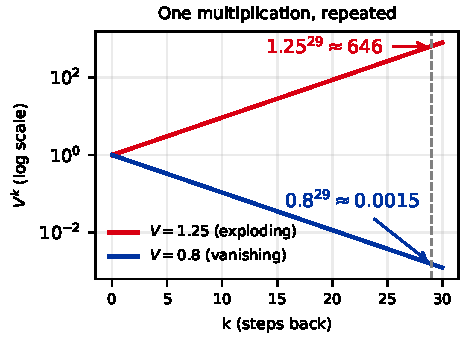
\includegraphics[width=\linewidth]{vanish_curve.pdf}\\[2pt]
      {\footnotesize \textcolor{armred}{Multiplication}: the disease. \textcolor{paramgreen}{Addition}: today's medicine.}
    \end{center}
  \end{columns}
\end{frame}

% 2026-10-23: Kargin Haghordum still (instructor's pick, the man who forgets how the chapter's
% Armenian line continues), same layout as 04_trees/20_advanced_boosting.tex's outline.
\begin{frame}{Outline}
  \begin{columns}[c]
    \column{0.54\textwidth}
    \tableofcontents
    \column{0.44\textwidth}
    \begin{center}
      \href{https://youtu.be/jcYTSHRiubE}{%
        
\includegraphics[width=\linewidth]{kargin_forgot_line.jpg}}\\[4pt]
      {\footnotesize\href{https://youtu.be/jcYTSHRiubE}%
        {\textcolor{armblue}{\underline{$\blacktriangleright$~Kargin Haghordum, ep.~24}}}}
    \end{center}
  \end{columns}
\end{frame}

% ================================================================
\section{LSTM: the additive fix}

\begin{frame}[plain]
  \vfill
  \begin{center}
    {\Large\color{popblue}\textbf{A memory highway}}\\[0.9em]
    \begin{minipage}{0.82\textwidth}\centering\small
      Hochreiter \& Schmidhuber's 1997 answer to the disease Hochreiter's own 1991
      thesis diagnosed.
    \end{minipage}
  \end{center}
  \vfill
\end{frame}

% 2026-10-15: Olah's chain enlarged to most of the line width (it was a 0.58-column
% thumbnail whose labels could not be read).
\begin{frame}{The cell state}
  \small
  The \textbf{Long Short-Term Memory} (\textbf{LSTM}; Hochreiter \& Schmidhuber, 1997) adds
  a second track alongside the hidden state $\mathbf{z}$: the \textbf{cell state}
  $\mathbf{c}$, the line along the top. At every step it is only lightly modified - a little
  is removed, a little is added.
  \begin{center}
    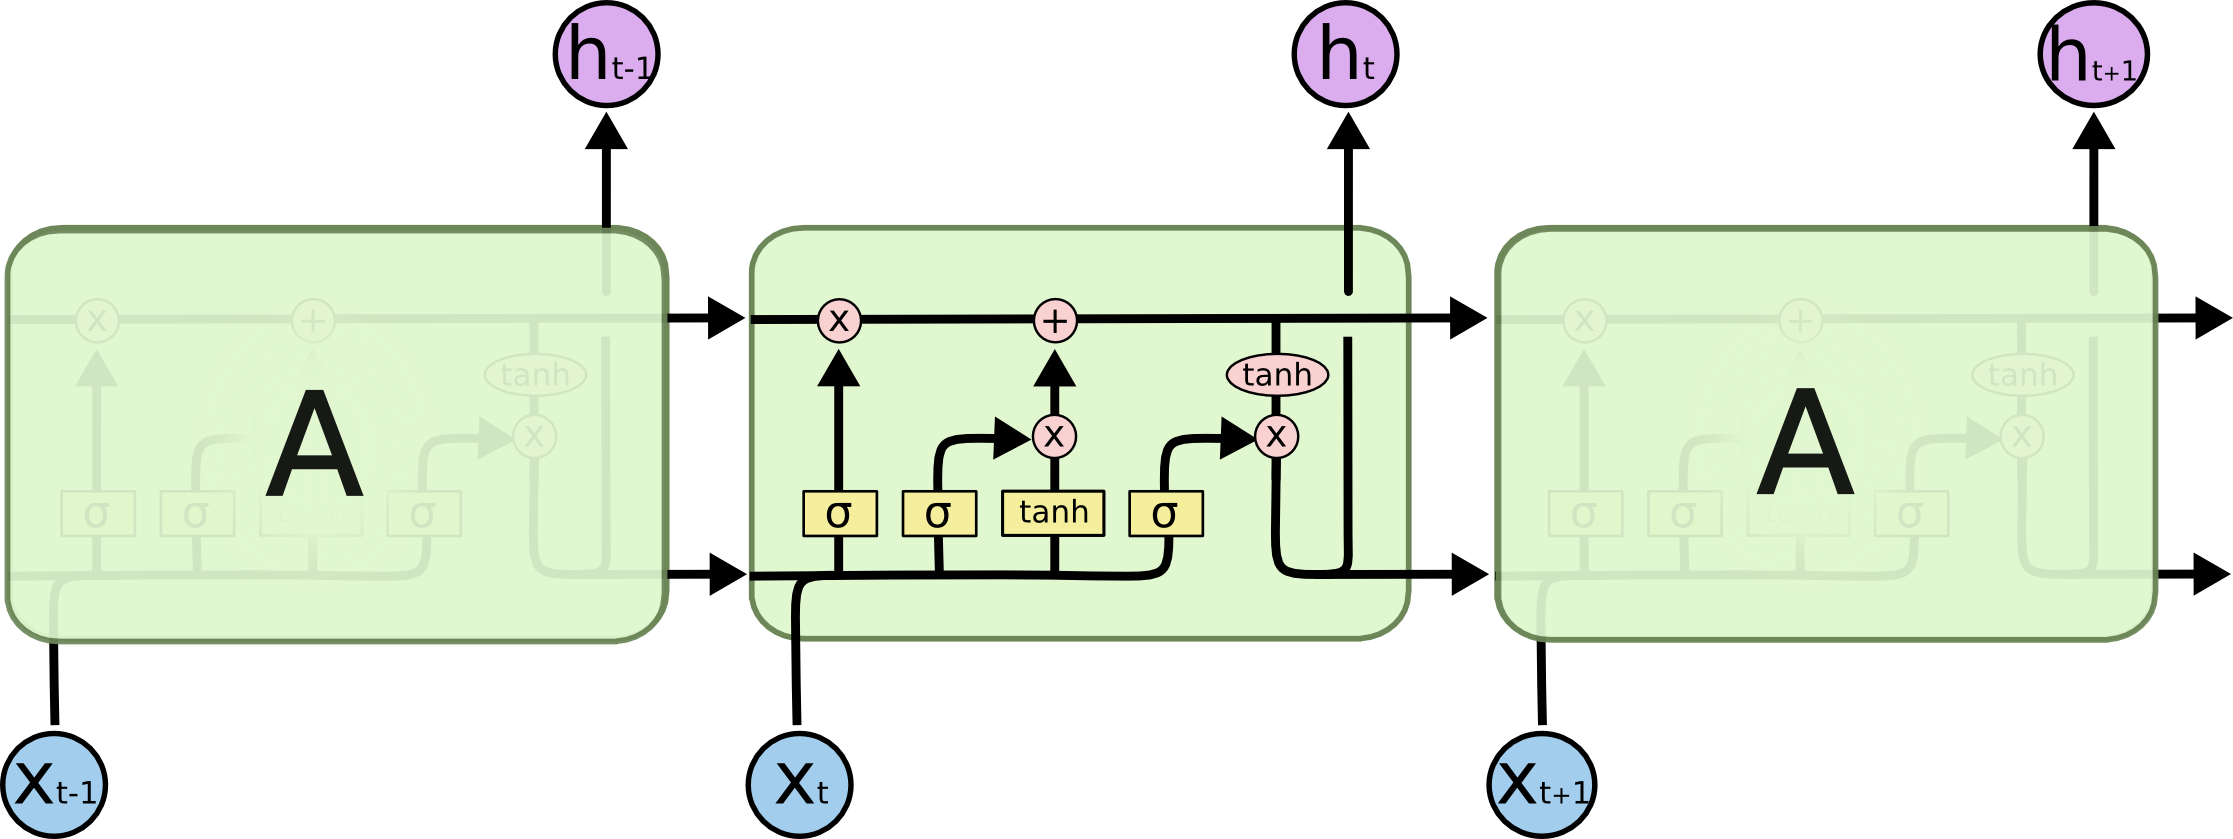
\includegraphics[width=0.80\linewidth]{olah_lstm_chain.png}
  \end{center}
  \vskip -4pt
  \begin{columns}[T]
    \column{0.55\textwidth}
    \fcolorbox{popblue}{popblue!6}{\parbox{0.95\linewidth}{\raggedright\footnotesize
      \textbf{Sorting-line metaphor}: the belt carries the box past every station; each
      worker only adds or removes a little. Nobody rebuilds the box at every station.}}
    \column{0.43\textwidth}
    {\footnotesize Every horizontal line is a full vector; circles are element-wise
    operations; yellow boxes are learned layers.}
  \end{columns}
\end{frame}

% 2026-10-15: the TikZ anatomy was a tangle of eight curved input wires with labels under
% the circles; redrawn as lstm_anatomy.pdf (l21_diagrams.py) with one input bus, Olah-style.
% The predict-first gate example moved to its own frame below.
\begin{frame}{Anatomy of one LSTM step}
  \footnotesize
  Three gates and one candidate, each computed from $\mathbf{x}^{[t]}$ and
  $\mathbf{z}^{[t-1]}$; each gate is a sigmoid vector in $(0,1)$ used as an
  \textbf{element-wise mask} ($\odot$).
  \begin{center}
    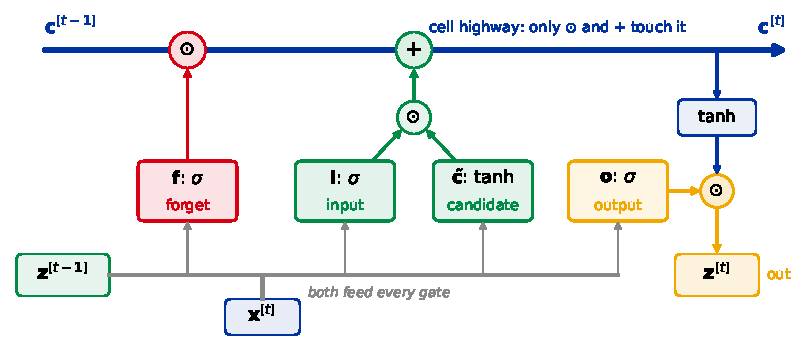
\includegraphics[width=0.92\linewidth]{lstm_anatomy.pdf}
  \end{center}
  \vskip -4pt
  {\scriptsize \textbf{Forget:} drop the old subject when a new one appears. \textbf{Input:}
  $\mathbf{i}$ says \emph{how much} to write, the candidate $\tilde{\mathbf{c}}$ says
  \emph{what} (a strong opinion word, say). \textbf{Output:} $\mathbf{c}$ is the cell's
  private memory; $\mathbf{z} = \mathbf{o}\odot\tanh(\mathbf{c})$ is the part it shows to the
  next step and the readout - only what is needed right now.\par}
\end{frame}

\begin{frame}{A gate is a soft switch}
  \begin{columns}[T]
    \column{0.5\textwidth}
    \small
    A gate is [41\_1]'s sigmoid neuron, rebranded: one number in $(0,1)$ per memory slot,
    multiplied element-wise into the cell.
    \vskip 6pt
    \textbf{Predict:} forget gate $[0.9,0.1]$ meets cell state $[2.0,-1.0]$ - what
    survives?
    \pause
    \vskip 6pt
    \fcolorbox{armorange}{armorange!12}{\parbox{0.95\linewidth}{\raggedright\small
      $[0.9,0.1]\odot[2.0,-1.0]=[1.8,-0.1]$: memory 1 survives almost untouched, memory 2
      is nearly wiped. Near 1 = keep, near 0 = erase, and the network picks the value at
      every step.}}
    \column{0.5\textwidth}
    \begin{center}
      \visible<2->{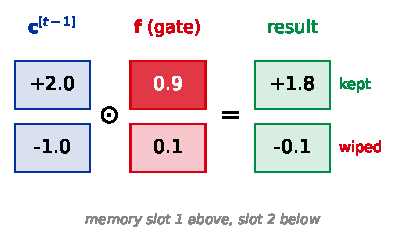
\includegraphics[width=\linewidth]{gate_mask.pdf}}
    \end{center}
  \end{columns}
\end{frame}

% 2026-10-23 (instructor: "why do we have c~, and why sigmoid?"). After the soft switch, so the
% gate-as-fraction idea is already on the table.
\begin{frame}{Why a candidate $\tilde{\mathbf{c}}$, and why sigmoid?}
  \begin{columns}[T]
    \column{0.5\textwidth}
    \small
    $\tilde{\mathbf{c}}$ is \textbf{[53]'s RNN step}, the same formula:
    \[
      \tilde{\mathbf{c}}^{[t]} = \tanh\big(\mathbf{W}^\top\mathbf{x}^{[t]}
        + \mathbf{V}^\top\mathbf{z}^{[t-1]} + \mathbf{b}\big)
    \]
    The vanilla RNN made this its new state: a full rewrite at every step, and that rewrite
    is the multiplication that starved the gradient. The LSTM treats it as a
    \textbf{proposal} and adds only a dose of it:
    \[
      \mathbf{c}^{[t]} = \mathbf{f}\odot\mathbf{c}^{[t-1]} + \mathbf{i}\odot\tilde{\mathbf{c}}^{[t]}
    \]
    Two questions, two small layers: \textbf{what} to write ($\tilde{\mathbf{c}}$) and
    \textbf{how much} of it ($\mathbf{i}$).
    \column{0.48\textwidth}
    \fcolorbox{armblue}{armblue!8}{\parbox{0.95\linewidth}{\raggedright\small
      \textbf{Sigmoid} for $\mathbf{f}$, $\mathbf{i}$, $\mathbf{o}$: a gate is a
      \textbf{fraction}, $0$ = shut, $1$ = open. Multiplying by a number in $(0,1)$ can only
      keep or shrink - never flip a sign, never blow up.}}
    \vskip 6pt
    \fcolorbox{armorange}{armorange!12}{\parbox{0.95\linewidth}{\raggedright\small
      \textbf{tanh} for $\tilde{\mathbf{c}}$: content needs a \textbf{sign}. "Sweet" pushes a
      mood slot up, "rotten" pushes it down; a sigmoid could only ever push up. The bound
      $(-1,1)$ keeps one step from writing a huge number.}}
    \vskip 6pt
    {\footnotesize Why not a hard 0/1 switch? Its slope is $0$ everywhere except at the jump,
    so backprop could never tune it. A sigmoid is a switch you can differentiate.\par}
  \end{columns}
\end{frame}

% 2026-10-20 (Sonnet student review: "why both i and c~? why an output gate?"). Numbers checked
% with a throwaway script: keep [1.8,-0.1], write [0.10,0.72], c [1.90,0.62],
% tanh(c) [0.956,0.551], z [0.908,0.028].
\begin{frame}{One full LSTM step, in numbers}
  \small
  The same two memory slots, now with every gate. Made-up gate values - a real cell computes
  each one from $\mathbf{x}^{[t]}$ and $\mathbf{z}^{[t-1]}$ with its own small layer:
  $\mathbf{f} = [0.9, 0.1]$, $\mathbf{i} = [0.2, 0.9]$, $\tilde{\mathbf{c}} = [0.5, 0.8]$,
  $\mathbf{o} = [0.95, 0.05]$. \textbf{(Click to advance.)}
  \vskip 6pt
  \begin{center}
    \renewcommand{\arraystretch}{1.5}
    \begin{tabular}{@{}r@{\quad}l@{}}
      \textcolor{armred}{\textbf{keep}} &
        $\mathbf{f}\odot\mathbf{c}^{[t-1]} = [0.9,\ 0.1]\odot[2.0,\ {-1.0}] = [1.8,\ {-0.1}]$ \\
      \onslide<2->{\textcolor{paramgreen}{\textbf{write}}} &
        \onslide<2->{$\mathbf{i}\odot\tilde{\mathbf{c}} = [0.2,\ 0.9]\odot[0.5,\ 0.8]
        = [0.10,\ 0.72]$} \\
      \onslide<3->{\textcolor{armblue}{\textbf{new cell}}} &
        \onslide<3->{$\mathbf{c}^{[t]} = \text{keep} + \text{write} = [1.90,\ 0.62]$} \\
      \onslide<4->{\textcolor{armorange}{\textbf{show}}} &
        \onslide<4->{$\mathbf{z}^{[t]} = \mathbf{o}\odot\tanh(\mathbf{c}^{[t]})
        = [0.95,\ 0.05]\odot[0.96,\ 0.55] = [0.91,\ 0.03]$} \\
    \end{tabular}
  \end{center}
  \vskip 4pt
  \onslide<5->{\fcolorbox{popblue}{popblue!6}{\parbox{0.97\linewidth}{\raggedright\small
    \textbf{Slot 1} keeps its memory and shows it. \textbf{Slot 2} drops the old $-1$,
    writes $0.72$ instead - and keeps it private: it holds $0.62$ but shows only $0.03$.
    $\mathbf{i}$ decides how much to write, $\tilde{\mathbf{c}}$ what, $\mathbf{o}$ who gets
    to see it.}}}
\end{frame}

% 2026-10-23 (instructor: "an example of what is learned, which weights"). Toy weights made up for
% readability; numbers from a throwaway script: sigma(3) = 0.9526, sigma(-3) = 0.047,
% sigma(2) = 0.881, tanh(2) = 0.964; c = 0.849, 0.809, 1.620; "rotten" instead of "sweet": -0.079.
\begin{frame}{What is learned, what is computed}
  \footnotesize
  A toy cell: \textbf{one} memory slot that tracks the review's mood, and each word comes in as
  two numbers, $\mathbf{x} = [\text{good}, \text{bad}]$ (no $\mathbf{V}$, no output gate). The
  weights are \textbf{made up} to be readable; training finds messier ones that do the same job.
  \vskip 4pt
  \begin{columns}[T]
    \column{0.42\textwidth}
    \fcolorbox{paramgreen}{paramgreen!8}{\parbox{0.95\linewidth}{\raggedright\footnotesize
      \textbf{Learned} by backprop, then fixed: 9 numbers.\\[4pt]
      $\tilde{c} = \tanh(\mathbf{W}^\top\mathbf{x} + b)$ \hfill \textcolor{gray}{which way?}\\
      $\mathbf{W} = [+2, -2]$, $b = 0$\\[4pt]
      $i = \sigma(\mathbf{W}_i^\top\mathbf{x} + b_i)$ \hfill \textcolor{gray}{opinion word?}\\
      $\mathbf{W}_i = [+5, +5]$, $b_i = -3$\\[4pt]
      $f = \sigma(\mathbf{W}_f^\top\mathbf{x} + b_f)$ \hfill \textcolor{gray}{keep 0.95}\\
      $\mathbf{W}_f = [0, 0]$, $b_f = +3$}}
    \column{0.56\textwidth}
    \textbf{Computed} fresh at every word, from those 9 numbers. Rule:
    $c \leftarrow 0.95\,c + i\,\tilde{c}$, starting from $c = 0$.
    \vskip 4pt
    \begin{center}
      \renewcommand{\arraystretch}{1.2}
      \begin{tabular}{@{}l c r r r@{}}
        word & $\mathbf{x}$ & $\tilde{c}$ & $i$ & new $c$ \\ \hline
        The \dots\ arrived & $[0, 0]$ & $0$ & $0.05$ & $0$ \\
        fresh & $[1, 0]$ & $+0.96$ & $0.88$ & $0.85$ \\
        and & $[0, 0]$ & $0$ & $0.05$ & $0.81$ \\
        sweet & $[1, 0]$ & $+0.96$ & $0.88$ & $\mathbf{1.62}$ \\ \hline
        \textcolor{armred}{rotten, not sweet} & $[0, 1]$ & \textcolor{armred}{$-0.96$} & $0.88$
          & \textcolor{armred}{$-0.08$} \\
      \end{tabular}
    \end{center}
  \end{columns}
  \vskip 4pt
  \fcolorbox{popblue}{popblue!6}{\parbox{0.97\linewidth}{\raggedright\footnotesize
    \textbf{Same input, two readings:} "sweet" and "rotten" open the gate equally and write
    opposite signs. A real cell learns the same kind of weights, as matrices - 1,152 numbers
    for a 16-slot cell - and nobody picks them by hand.}}
\end{frame}

% 2026-10-15 (instructor): "gate story on the Goris sentence" - the LSTM handles the sentence
% L20's fixed-window frame could not. Gate values are illustrative (labelled on the figure);
% the cell values are computed with c = f*c + i*cand and asserted in l21_diagrams.py.
\begin{frame}{Watching one memory slot}
  \small
  The sentence from [53]'s fixed-window frame, read by an LSTM. One slot of its cell has
  learned one job: remember whether the subject is plural. The gate values are
  \textbf{made up} to show the mechanism - a trained cell is messier (measured results in a
  few frames). \textbf{(Click to advance.)}
  \begin{center}
    \only<1>{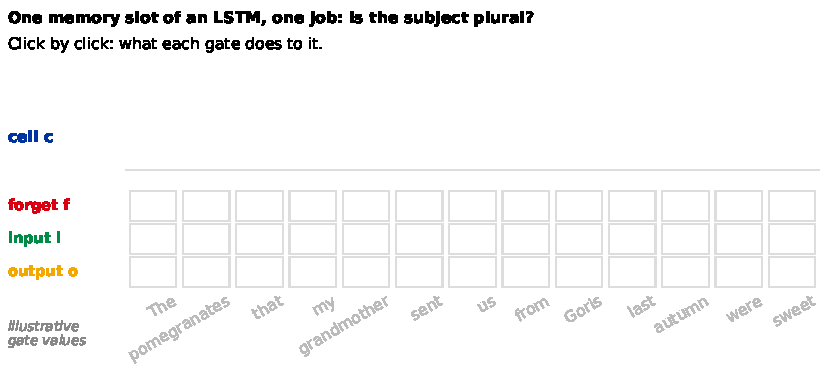
\includegraphics[width=0.9\linewidth]{gate_story_0.pdf}}%
    \only<2>{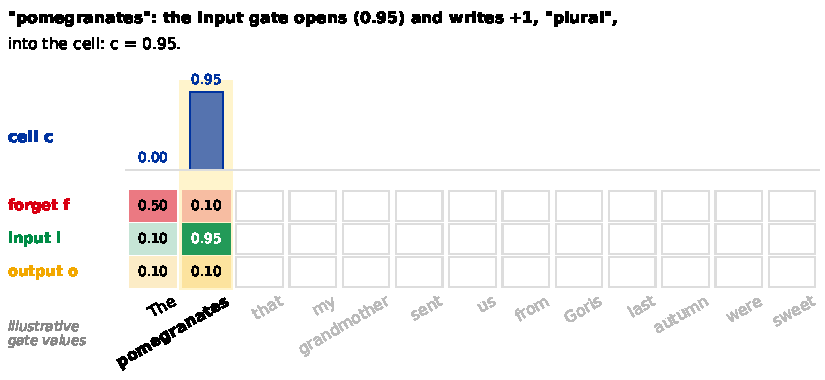
\includegraphics[width=0.9\linewidth]{gate_story_1.pdf}}%
    \only<3>{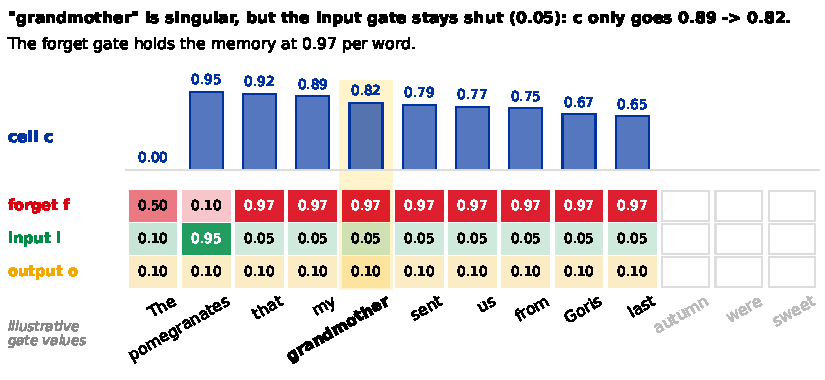
\includegraphics[width=0.9\linewidth]{gate_story_2.pdf}}%
    \only<4>{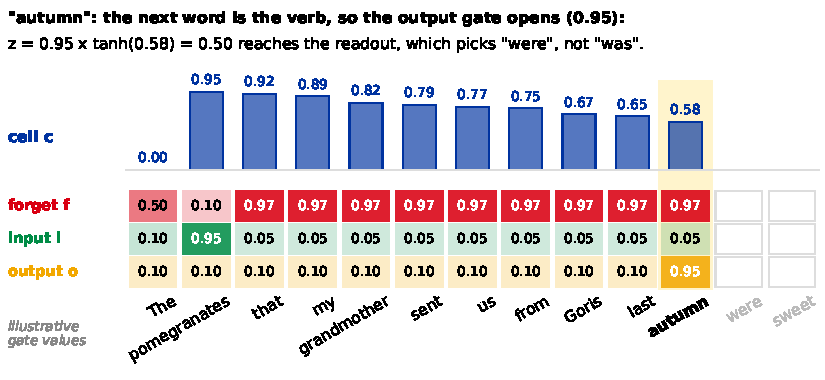
\includegraphics[width=0.9\linewidth]{gate_story_3.pdf}}%
    \only<5>{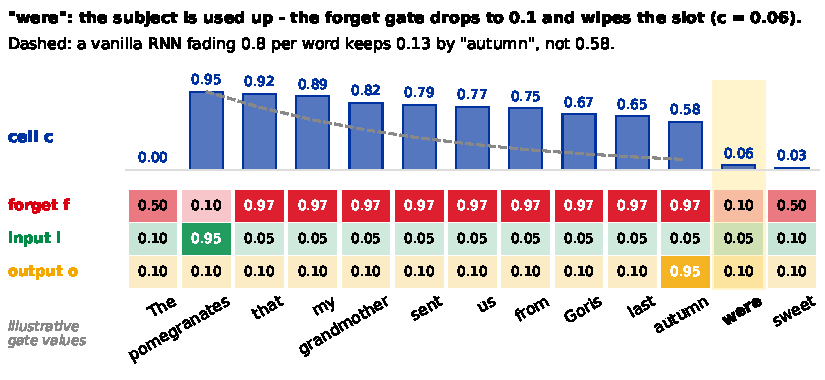
\includegraphics[width=0.9\linewidth]{gate_story_4.pdf}}%
  \end{center}
\end{frame}

\begin{frame}{For the record: the four equations}
  \footnotesize\textcolor{gray}{Reference, not exam material - shown once.}
  \vskip 2pt
  % 2026-10-15: boxes stacked relative to each other (they were placed at fixed y and the
  % two-line input box overlapped the forget box); the output box gets its second line.
  \begin{center}
    \begin{tikzpicture}[scale=0.86, transform shape,
        eqbox/.style={rounded corners=6pt, text width=11cm, align=left, inner sep=7pt,
          font=\normalsize}]
      \node[eqbox, draw=armred, fill=armred!8] (fg) at (0, 0) {
        \textbf{\textcolor{armred}{Forget gate:}} \quad
        $\mathbf{f}^{[t]} = \sigma\!\big(\mathbf{W}_f^\top\xv^{[t]} + \mathbf{V}_f^\top\mathbf{z}^{[t-1]} + \mathbf{b}_f\big)$
      };
      \node[eqbox, draw=paramgreen, fill=paramgreen!8, anchor=north] (ig)
        at ([yshift=-5pt]fg.south) {
        \textbf{\textcolor{paramgreen}{Input gate:}} \quad
        $\mathbf{i}^{[t]} = \sigma\!\big(\mathbf{W}_i^\top\xv^{[t]} + \mathbf{V}_i^\top\mathbf{z}^{[t-1]} + \mathbf{b}_i\big)$
        \\[3pt] \phantom{\textbf{Input gate:}} \quad
        $\tilde{\mathbf{c}}^{[t]} = \tanh\!\big(\mathbf{W}^\top\xv^{[t]} + \mathbf{V}^\top\mathbf{z}^{[t-1]} + \mathbf{b}\big)$
      };
      \node[eqbox, draw=armblue, fill=armblue!8, anchor=north] (cu)
        at ([yshift=-5pt]ig.south) {
        \textbf{\textcolor{armblue}{Cell update:}} \quad
        $\mathbf{c}^{[t]} = \mathbf{f}^{[t]} \odot \mathbf{c}^{[t-1]} \;+\; \mathbf{i}^{[t]} \odot \tilde{\mathbf{c}}^{[t]}$
      };
      \node[eqbox, draw=armorange, fill=armorange!8, anchor=north] (og)
        at ([yshift=-5pt]cu.south) {
        \textbf{\textcolor{armorange}{Output gate:}} \quad
        $\mathbf{o}^{[t]} = \sigma\!\big(\mathbf{W}_o^\top\xv^{[t]} + \mathbf{V}_o^\top\mathbf{z}^{[t-1]} + \mathbf{b}_o\big)$
        \\[3pt] \phantom{\textbf{Output gate:}} \quad
        $\mathbf{z}^{[t]} = \mathbf{o}^{[t]} \odot \tanh(\mathbf{c}^{[t]})$
      };
      \node[draw=popblue, fill=popblue!6, rounded corners=6pt, text width=12.5cm,
        align=center, inner sep=7pt, font=\small, anchor=north] at ([yshift=-8pt]og.south) {
        The punchline: $\mathbf{c}^{[t]} = \mathbf{f}^{[t]}\odot\mathbf{c}^{[t-1]} + \dots$
        is \textbf{additive} - gradients flow through the cell state with minimal
        decay. ResNet solved \emph{depth} with addition in 2015; LSTM solved
        \emph{time} with addition in 1997 - same medicine, 18 years earlier.
      };
    \end{tikzpicture}
  \end{center}
\end{frame}

% 2026-09-22 addition: the one derivative that explains WHY the highway works - intuition
% level, no full LSTM backprop (instructor: LSTM is context, not curriculum).
\begin{frame}{Why addition keeps the gradient alive}
  \small
  Follow the gradient backwards along the highway only (ignore the paths through the
  gates). One line of calculus:
  \[
    \mathbf{c}^{[t]} = \mathbf{f}^{[t]}\odot\mathbf{c}^{[t-1]}
      + \mathbf{i}^{[t]}\odot\tilde{\mathbf{c}}^{[t]}
    \quad\Longrightarrow\quad
    \frac{\partial \mathbf{c}^{[t]}}{\partial \mathbf{c}^{[t-1]}}
      = \mathrm{diag}\big(\mathbf{f}^{[t]}\big)
  \]
  The other paths back run through the gates and their weight matrices, and those do fade
  like an RNN's. The highway does not have to - and one path that survives is enough to
  carry the signal.
  \vskip 4pt
  \begin{columns}[T]
    \column{0.48\textwidth}
    \fcolorbox{armred}{armred!8}{\parbox{0.95\linewidth}{\raggedright\small
      \textbf{Vanilla RNN ([53]):} each step multiplies by
      $\mathbf{D}^{[t-1]}\mathbf{V}^\top$ - the \emph{same} matrix every step, whether or
      not the memory matters. Its size decides the fate of everything.}}
    \column{0.48\textwidth}
    \fcolorbox{paramgreen}{paramgreen!8}{\parbox{0.95\linewidth}{\raggedright\small
      \textbf{LSTM highway:} each step multiplies by $\mathbf{f}^{[t]}$, which the network
      \emph{recomputes} every step, per slot: $\approx 1$ to hold, $\approx 0$ to wipe.
      Close to 1 matters: $0.97^{100} \approx 0.05$, $0.99^{100} \approx 0.37$
      (vanilla: $0.8^{100} \approx 2\cdot 10^{-10}$).}}
  \end{columns}
  \vskip 6pt
  {\footnotesize \textbf{History:} the 1997 LSTM had \emph{no} forget gate - a "constant
  error carousel" with factor exactly $1$. On long, unsegmented input its cell state kept
  growing until the network broke down; the forget gate (Gers, Schmidhuber \& Cummins,
  2000) lets it reset.\par}
\end{frame}

% 2026-09-22: figure replaced. The old gradient_flow_comparison.pdf showed no LSTM advantage
% (reported honestly, but it left the frame's own question unanswered). memory_highway.py
% measures the mechanism (sensitivity at init vs forget-gate bias) and the outcome
% (first-token recall, 2 seeds); every claim below is read off results/memory_highway.json.
\begin{frame}{Does it work? Measured}
  \vskip -4pt
  \begin{center}
    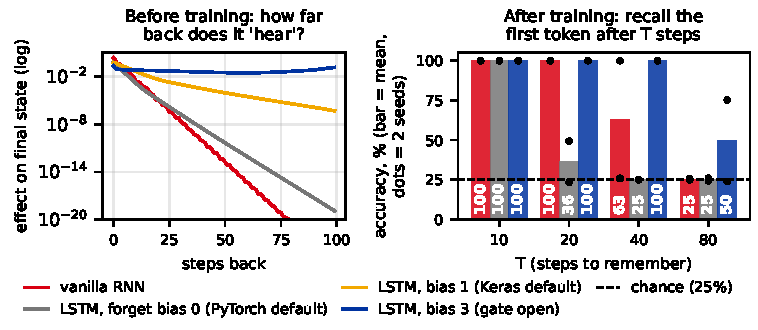
\includegraphics[width=0.92\linewidth]{memory_highway.pdf}
  \end{center}
  \vskip -6pt
  % 2026-10-15: "coin flip" and "succeeds" replaced by what the JSON says per seed:
  % RNN T=40 = 100% (seed 509) / 26% (seed 510); LSTM bias 3 T=80 = 75% / 24%.
  {\footnotesize \textbf{Left}, before training: an input 40 steps back barely moves a
  vanilla RNN or a half-shut LSTM (bias 0); bias 1 decays slower; open gates (bias 3) still
  count at 100. \textbf{Right}, same budget: the open-gate LSTM solves $T \le 40$ in 100
  steps; at $T = 40$ the RNN solves one seed of two, at 80 neither, and even the open-gate
  LSTM reaches only 75\% on one seed. Addition makes long memory \emph{learnable}, not free.}
\end{frame}

\begin{frame}[fragile]{The price, and one gotcha}
  \begin{itemize}
    \item \textbf{Price:} 4 weight sets instead of 1. Our $d_x{=}1,d_h{=}16$ vanilla
      cell: $16\,(\mathbf{W}) + 256\,(\mathbf{V}) + 16\,(\mathbf{b}) = 288$ params. LSTM:
      $4\times288=\mathbf{1{,}152}$. (PyTorch's \texttt{nn.LSTM} keeps two bias vectors,
      so it reports 1,216.)
    \item \textbf{Gated Recurrent Unit} (\textbf{GRU}; Cho et al., 2014): a streamlined
      2-gate cousin (3 weight sets), similar results - the lighter default.
    \item \textbf{Gotcha:} the measured frame's "gate starts open" (bias 3) is a one-line
      choice. The gate starts at $\sigma(\text{bias})$: $\sigma(0) = 0.5$ halves the memory
      every step, $\sigma(3) \approx 0.95$ keeps it. Keras adds $+1$ to the forget-gate bias
      by default; \textbf{PyTorch does not}:
  \end{itemize}
  \small
\begin{verbatim}
lstm = nn.LSTM(d_in, hidden)
# PyTorch stacks the gates: input, forget, cell, output
lstm.bias_ih_l0.data[hidden:2 * hidden].fill_(1.0)  # forget gate
\end{verbatim}
  \fcolorbox{armorange}{armorange!12}{\parbox{0.97\linewidth}{\small
    Same lesson as [45]'s initialization frames: where training \emph{starts} can decide
    whether it gets anywhere at all.}}
\end{frame}

\begin{frame}{Published 1997, everywhere by 2016}
  % 2026-10-15: TikZ timeline (hyphenated, wrapped labels) redrawn as lstm_timeline.pdf.
  \small
  \begin{center}
    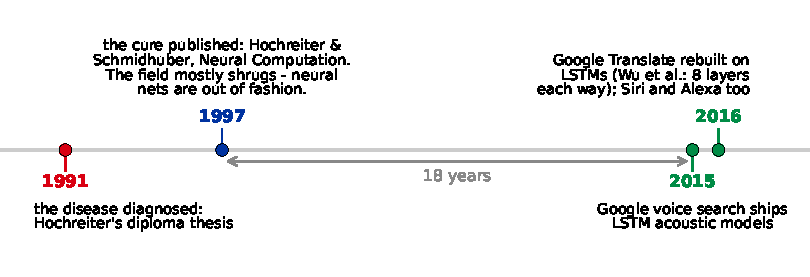
\includegraphics[width=\linewidth]{lstm_timeline.pdf}
  \end{center}
  \vskip -4pt
  \fcolorbox{paramgreen}{paramgreen!8}{\parbox{0.97\linewidth}{\small
    \textbf{18 years} from publication to running in everyone's pocket - and one of
    the most-cited AI papers ever (80{,}000+ citations). When a 2010s product said
    "powered by neural networks", the network was very often an LSTM.}}
  \vskip 3pt
  {\footnotesize Fine print, for next chapter: 2016's Google Translate already carried
  an \emph{attention} link between its encoder and decoder - the idea beyond LSTM was
  creeping in even at LSTM's moment of triumph.}
\end{frame}

% 2026-10-03: the section "Tokens: how text becomes numbers" (transition, tokenization
% trilemma, subwords on a real tokenizer, the Armenian tax, embeddings) moved to the LLM
% chapter (ml/LLM_CHAPTER_PLAN.md, LLM-1 and LLM-7); "One-hot and its poverty" moved to L20.
% DECISIONS #64. Last version with the section: git show 6013bcc:ml/ch7_rnn/54_road_to_attention.tex

% 2026-10-23 (instructor, DECISIONS #95): the section "Language modeling" (transition, the
% objective, the GRU's next-letter bars, the generation loop, the surname demo, the loss curve)
% removed - next-token prediction and the generation loop are taught later, in the LLM chapter.
% Figures surname_*.pdf and py_src/surname_gru.py kept. Last version with the section:
% git show a001201:ml/13_rnns/L21_road_to_attention.tex

% ================================================================
\section{Seq2Seq and the wall}

\begin{frame}[plain]
  \vfill
  \begin{center}
    {\Large\color{popblue}\textbf{Two networks, one vector between them}}\\[0.9em]
    \begin{minipage}{0.82\textwidth}\centering\small
      Translation needs a different-length output. Here is the classic fix.
    \end{minipage}
  \end{center}
  \vfill
\end{frame}

% 2026-10-15: the Alammar still (a thumbnail with no words in it) replaced by seq2seq.pdf,
% the chapter's own translation pair drawn word by word (l21_diagrams.py).
\begin{frame}{Encoder-decoder}
  \small
  Translation needs different input and output lengths. Fix: an \textbf{encoder} LSTM reads
  the source; its last state is ONE \textbf{context vector} $C$. A \textbf{decoder} LSTM
  starts from $C$ (and, in Cho et al.'s version, gets it again at every step, dashed) and
  writes the target one word at a time - each written word fed back in as its next input.
  \begin{center}
    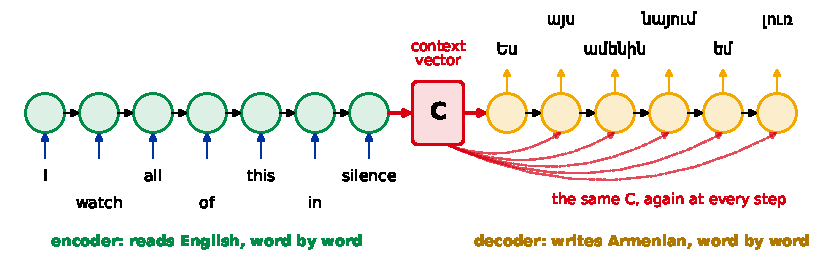
\includegraphics[width=\linewidth]{seq2seq.pdf}
  \end{center}
  \vskip -6pt
  {\footnotesize Running example: "I watch all of this in silence, and the connoisseurs
  speak inside me." goes in, and the decoder writes the chapter's Armenian line from [53]
  (first half shown). The 2014 recipe that made neural machine translation real: Sutskever,
  Vinyals \& Le (2014); Cho et al. (2014).}
\end{frame}

\begin{frame}{The bottleneck}
  \footnotesize
  \textbf{Predict:} the 42-word complaint review ([53]'s shoehorn-hacks frame - it lost
  its verdict to truncation already) squeezed into a single 300-dim context vector.
  What goes wrong?
  \pause
  % 2026-10-15: the TikZ funnel's boxes overlapped; redrawn as bottleneck.pdf, the two
  % verdicts and the LSTM box moved into the slide text.
  \begin{center}
    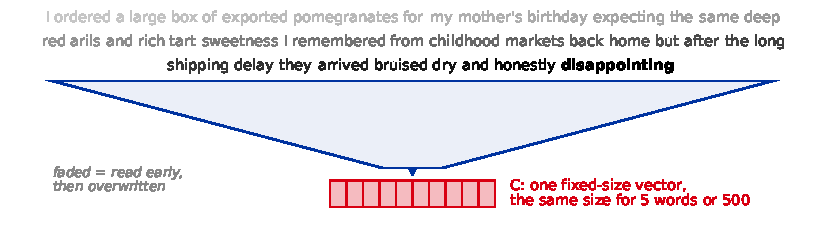
\includegraphics[width=0.94\linewidth]{bottleneck.pdf}
  \end{center}
  \vskip -6pt
  \begin{columns}[T]
    \column{0.49\textwidth}
    \fcolorbox{armred}{armred!8}{\parbox{0.95\linewidth}{\raggedright\footnotesize
      \textbf{Lost:} early words get overwritten as the state updates - "expecting",
      "childhood markets" fade first.}}
    \column{0.49\textwidth}
    \fcolorbox{armorange}{armorange!12}{\parbox{0.95\linewidth}{\raggedright\footnotesize
      \textbf{Fixed capacity:} 5 words or 500, the same-size $C$ must hold them all.}}
  \end{columns}
  \vskip 4pt
  \fcolorbox{popblue}{popblue!6}{\parbox{0.97\linewidth}{\centering\footnotesize
    \textbf{And the LSTM does NOT save us}: the cell state is still one fixed-size vector.
    The fix for \emph{fading} memory did not fix \emph{compressed} memory.}}
\end{frame}

% 2026-10-03: the alignment frame (instructor: "I like that real insight point being emphasized").
% Grid from py_src/alignment_grid.py; the alignment itself is hand-made - see that script.
% Does not name the answer (the cliffhanger lock still holds): "alignment" is the classical
% machine-translation word, used here only for what each output word needs.
\begin{frame}{The real problem: every step gets the same $C$}
  \begin{columns}[T]
    \column{0.55\textwidth}
    \begin{center}
      \only<1>{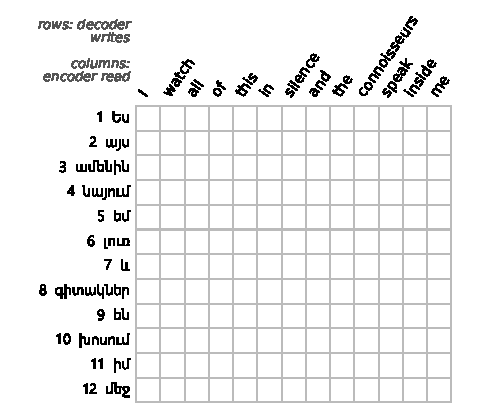
\includegraphics[width=\linewidth]{alignment_grid_0.pdf}}%
      \only<2->{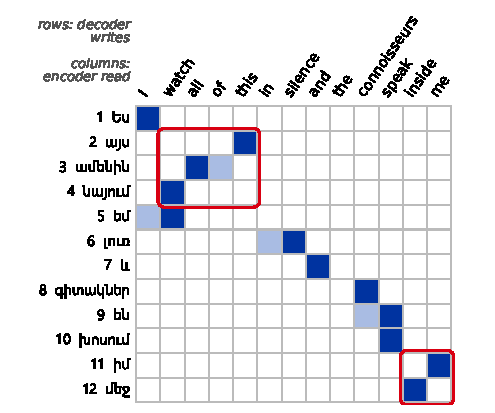
\includegraphics[width=\linewidth]{alignment_grid_1.pdf}}%
    \end{center}
    \column{0.45\textwidth}
    \small
    So just make $C$ bigger? First look at what the decoder actually \emph{needs}.
    \vskip 4pt
    \textbf{Predict:} the decoder writes the Armenian line one word per row. For each row,
    which English words does it need?
    \pause
    \vskip 6pt
    Each row needs \textbf{one or two} words - a \textbf{different} few every time, and not
    even in order: rows 2-4 run backwards ("this all watch"), and so do rows 11-12 ("my
    inside").
    \vskip 6pt
    \fcolorbox{armred}{armred!8}{\parbox{0.95\linewidth}{\small
      Seq2seq hands \textbf{every} step the \textbf{same} $C$. The deeper problem is not
      that $C$ is small: each step needs a \textbf{different part} of the input, and
      nothing lets the decoder go and get it.}}
  \end{columns}
\end{frame}

% 2026-09-22 addition: the second reason recurrence lost - sequential compute. Quote verified
% verbatim against arXiv 1706.03762v7, Introduction. Deliberately does NOT name the answer
% (the cliffhanger lock below still holds).
\begin{frame}{The second wall: one step at a time}
  \small
  Even a perfect LSTM has one more problem, and it is about \textbf{speed}, not memory:
  $\mathbf{z}^{[t]}$ needs $\mathbf{z}^{[t-1]}$, which needs $\mathbf{z}^{[t-2]}$ ... Step
  $t$ cannot start until step $t-1$ has finished.
  \vskip 4pt
  \begin{center}
    \begin{tikzpicture}[font=\scriptsize, >=Latex,
        n/.style={draw, circle, minimum size=0.62cm, fill=paramgreen!18}]
      \foreach \i/\x in {1/0,2/1.3,3/2.6}
        \node[n] (z\i) at (\x,0) {$z_{\i}$};
      \node (dots) at (3.9,0) {$\cdots$};
      \node[n] (zN) at (5.2,0) {$z_{1000}$};
      \draw[->, thick] (z1) -- (z2); \draw[->, thick] (z2) -- (z3);
      \draw[->, thick] (z3) -- (dots); \draw[->, thick] (dots) -- (zN);
      \node[armred, align=left, anchor=west] at (6.1,0)
        {1{,}000 tokens $=$ 1{,}000 steps\\in a queue, one after another};
    \end{tikzpicture}
  \end{center}
  \vskip 2pt
  \begin{itemize}
    \item The GPUs from [42] want thousands of \emph{independent} multiply-adds at once.
      A recurrence hands them one small step at a time - most of the chip waits.
    \item The authors of the paper that ended the RNN era put it plainly: "This
      inherently sequential nature precludes parallelization within training examples"
      (Vaswani et al., 2017).
  \end{itemize}
  \vskip 4pt
  \fcolorbox{armblue}{armblue!8}{\parbox{0.97\linewidth}{\small
    Two walls, then: the \textbf{bottleneck} (one vector, the same for every step, must
    hold everything) and the \textbf{queue} (one step at a time). The next chapter takes
    them down with two moves: let the decoder look back at every encoder state (the
    bottleneck), and drop the recurrence so all words are read at once (the queue).}}
\end{frame}

\begin{frame}{The cliffhanger}
  \small
  What if the decoder could look back at \emph{all} the encoder states - and learn
  \emph{where} to look, a different place for every word it writes?
  % 2026-10-15: the all-to-all dashed TikZ arrows merged into a grey smear; redrawn as
  % cliffhanger.pdf - dashed "?" lines from every encoder state to the ONE decoder step being
  % written now. Still unlabeled: the answer is not named here (locked).
  \begin{center}
    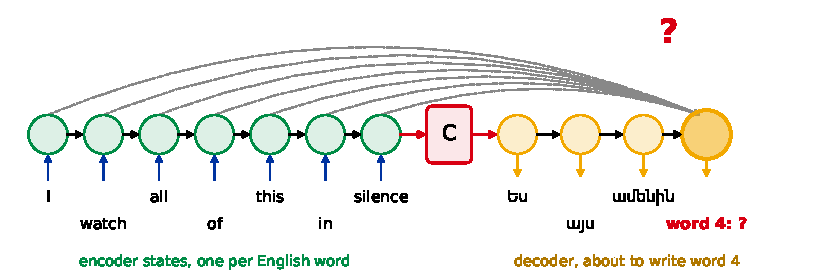
\includegraphics[width=\linewidth]{cliffhanger.pdf}
  \end{center}
  \vskip -4pt
  \fcolorbox{popblue}{popblue!6}{\parbox{0.97\linewidth}{\small
    That question has a name. It was answered between 2014 and 2017, and it ends this
    course's pre-history of sequence models. Next chapter: attention and
    transformers.}}
\end{frame}

% ================================================================
\section{Epilogue: recurrence in 2026}

\begin{frame}{Recurrence, retirement, and a comeback}
  \begin{center}
    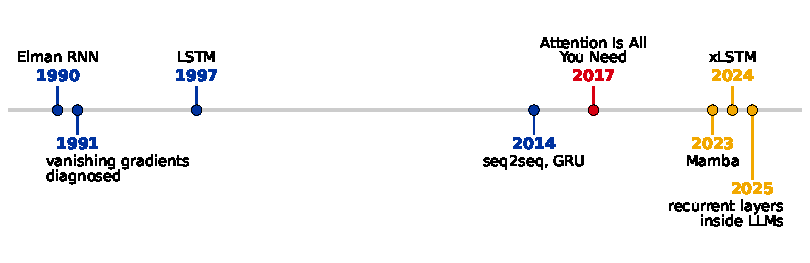
\includegraphics[width=0.98\linewidth]{rnn_timeline.pdf}
  \end{center}
  \small
  2017's transformer retired RNNs from mainstream NLP. But recurrence is back: several
  2025-26 LLMs run most of their layers as a fixed-size recurrent state with a learned
  \emph{decay} gate - today's forget gate. Why it came back makes sense only once you know
  what it replaced: the LLM chapter.
\end{frame}

% ================================================================
\section*{Recap}

\begin{frame}{Recap}
  \begin{itemize}
    \item Length varies, memory fades ([53]) $\to$ LSTM fixes fading with an
      \textbf{additive} cell state - same medicine as ResNet, 18 years earlier - at
      4$\times$ the parameter cost. Its gates decide, per memory slot, what to write, keep
      and release.
    \item \textbf{Seq2seq} squeezes the whole source sentence into one vector $C$ and hands
      \textbf{every} output step that \textbf{same} $C$ - while each step needs a
      \textbf{different} part of the input. And any recurrence runs \textbf{one step at a
      time}.
  \end{itemize}
  \vskip 6pt
  \fcolorbox{paramgreen}{paramgreen!8}{\parbox{0.97\linewidth}{
      \textbf{Next:} the LLM chapter. It starts where text enters the model - what exactly is
      a token? - and then answers today's question: let the decoder look back at everything
      and take a different part for each word it writes. That is attention (LLM-3); dropping
      the recurrence altogether also removes the one-step-at-a-time queue.}}
\end{frame}

\end{document}

% ================================================================
% Provenance:
%   Deck: L21 The Road to Attention: LSTM, Tokens and the Bottleneck (13_rnns). Built
%   2026-07-13 from 54_road_to_attention_OUTLINE.md (BUILD-READY) + RNN_CHAPTER_PLAN.md,
%   following 53_rnn_foundations.tex as the style exemplar (anatomy-frame idiom, ANIM
%   \only<n> pattern, callout boxes, [plain] transitions, footer, Provenance format).
%
%   INSTRUCTOR SCOPE CHANGE (mid-build, 2026-07-13): no real training runs, no
%   dataset/model downloads. The outline's char-LSTM corpus fetch (Wikisource
%   Tumanyan/Charents), the GloVe embedding subset, and the tiktoken Armenian-tax panel
%   were each re-scoped or replaced -- full accounting in 54_DECISIONS.md.
%
%   Chapter constants reused verbatim (locked in L20): review sentence "The
%   pomegranates arrived fresh and sweet."; the Armenian line (py_src/data/
%   armenian_line.txt); the 42-word complaint review (py_src/pad_truncate.py's
%   REVIEWS dict); toy-net forward/reversed scores 0.38/0.82 (forward_pass_anim.py).
%   New chapter constants (this deck): English gloss "I watch all of this in silence,
%   and the connoisseurs speak inside me."; char-LM ANIM word Պանիր; gate-mask
%   micro-example [0.9,0.1] (*) [2.0,-1.0] = [1.8,-0.1] (verified with a throwaway
%   script before typesetting).
%
%   Sources consulted (REDERIVE, read-only, our own z/c/W/V notation throughout):
%   LMU I2DL rnn/slides-modernrnn.tex (LSTM cell-state idea, gate intuitions incl. the
%   gender-pronoun forget-gate example -- compressed to intuition level, no 9-click
%   equation buildup, no GRU derivation); rnn/slides-applications.tex (LM probability
%   factorization, the character-by-character "hello" click-sequence IDEA rebuilt on
%   Պանիր instead, word-embeddings framing, encoder-decoder + context vector).
%
%   OWN-TEX (misc/dl4nlp/01_pre_transformer.tex, per the chapter plan's whitelist;
%   colors swapped sampred/warnred/orange1/violet1 -> armred/armblue/armorange/
%   paramgreen for in-deck consistency, matching L20's item-5 precedent):
%   the gate-equations frame (~586-617) -> "For the record: the four equations."
%   The bottleneck frame (~802-838) -> "The bottleneck" (funnel + lost/fixed-capacity
%   boxes), re-worded around the 42-word review instead of the original's fox sentence.
%   The memory-highway frame (~535-581) informed the "The cell state" sorting-line
%   framing, but the WEB-IMG (Olah) diagram was used instead of this OWN-TEX diagram
%   for the actual figure (see WEB-IMG note below) -- the OWN-TEX seq2seq frame
%   (~721-797) was NOT used verbatim; the cliffhanger's dashed-arrow TikZ is a fresh
%   adaptation of its encoder/decoder/context-vector node layout, not a copy.
%   misc/dl4nlp/03_tokenization.tex was read before writing Section 2 (three-levels
%   framing, OOV problem) to preview rather than contradict ch8's future BPE deep dive.
%
%   WEB-IMG (fig/borrowed/, no credit lines per standing policy):
%   olah_lstm_chain.png <- https://colah.github.io/posts/2015-08-Understanding-LSTMs/
%   img/LSTM3-chain.png ("Understanding LSTM Networks", Chris Olah, 2015) -- used for
%   "The cell state" in place of the OWN-TEX memory-highway diagram (reads better at
%   16:9, per the outline's "pick whichever reads better" instruction).
%   alammar_seq2seq_still.png <- a still FRAME extracted with ffmpeg (timestamp ~8s)
%   from https://jalammar.github.io/images/seq2seq_3.mp4, one of the animated stills
%   on Jay Alammar's "Visualizing A Neural Machine Translation Model" post -- the site
%   now serves this content as .mp4, not .png, so a representative frame was captured
%   instead of a direct image download (logged as a build decision). The generic
%   input/encoder/decoder/output-triangles version was chosen over the
%   French-source variant (seq2seq_4) because the latter's frames never show both
%   source and target text simultaneously (the animation types one at a time), which
%   would have looked broken as a static still.
%
%   Figures (py_src -> fig, ma venv, seed 509): gradient_flow.py (MODIFIED -- added a
%   quick comparison re-run, TRAIN_STEPS_QUICK=1200, emitting NEW file
%   gradient_flow_comparison.pdf; gradient_flow_vanilla.pdf and
%   gradient_flow_vanilla_lstm.pdf are UNTOUCHED, verified byte-identical
%   before/after this build); tokenizer_demo.py (real tiktoken cl100k_base measurements
%   -- tokenizer_panel1/2/3.pdf); embedding_2d.py (ILLUSTRATIVE hand-placed schematic
%   -- embedding_2d.pdf); charlm_anim.py (ILLUSTRATIVE next-char bars on Պանիր --
%   charlm_anim_0..5.pdf); charlm_generate.py (ILLUSTRATIVE typical-progression panels
%   -- charlm_gen_0..4.pdf -- and a schematic loss curve, charlm_loss.pdf);
%   rnn_timeline.py (real, web-verified facts -- rnn_timeline.pdf; no
%   ml/12_cnn/py_src/timeline_ribbon.py exists in this repo to copy from, so this is a
%   fresh ribbon in the same house visual language). vanish_curve.pdf reused verbatim
%   from L20 for the cold open (no regeneration needed).
%
%   Epilogue facts web-verified at build (2026-07-13): Mamba (Gu & Dao, arXiv
%   2312.00752, 2023); xLSTM (Beck et al., NeurIPS 2024 spotlight, arXiv 2405.04517,
%   Sepp Hochreiter listed as senior/last author); GRU (Cho et al., arXiv June 2014,
%   "Learning Phrase Representations using RNN Encoder-Decoder..."); seq2seq
%   (Sutskever, Vinyals & Le, NeurIPS 2014, arXiv 1409.3215); "Attention Is All You
%   Need" (Vaswani et al., NeurIPS 2017, arXiv 1706.03762). All match the outline's
%   claims verbatim -- no corrections needed. Links verified live: tiktokenizer.vercel.
%   app, projector.tensorflow.org, karpathy.github.io/2015/05/21/rnn-effectiveness/.
%
%   REVISION 2026-09-06 (instructor request: add historic context): transition +
%   cell-state frames now name Hochreiter & Schmidhuber, with Long Short-Term Memory
%   (LSTM) expanded on first body use; GRU expanded (Gated Recurrent Unit) and
%   corrected from "3-gate cousin" to 2-gate / 3-weight-set; NEW frame "Published
%   1997, everywhere by 2016" (1991 thesis -> 1997 paper -> 2015 Google voice search
%   LSTM acoustic models -> 2016 Google Translate on LSTMs, Wu et al.; 80,000+
%   citations; footnote foreshadows the attention link already inside 2016's
%   Translate); encoder-decoder frame cites Sutskever, Vinyals & Le 2014 + Cho et
%   al. 2014; rnn_timeline.py extended back to 1990 (Elman) + 1991 (Hochreiter
%   diagnosis), YEAR_MIN 1996 -> 1987, title now 1990-2026. All facts web-verified
%   2026-09-06 (Google voice search LSTM: Google Research blog, Sept 2015; Google
%   Translate: arXiv 1609.08144, 8 encoder + 8 decoder LSTM layers with attention).
%
%   Key decisions, the instructor scope change, and open questions: logged in
%   54_DECISIONS.md.
%
%   REVISION 2026-09-22 (pre-delivery pedagogy pass, instructor away - autonomous):
%   - "A gate is L14's sigmoid" -> [41_1] (LMU 03_single-neuron, sigmoid neuron).
%   - NEW "Why addition keeps the gradient alive": d c_t / d c_{t-1} = diag(f_t) along the
%     highway vs L20's D V^T; history line - the 1997 LSTM had no forget gate (constant
%     error carousel), added by Gers, Schmidhuber & Cummins 2000 (web-verified).
%   - "Does it work? Proof + price" REOPENS the 2026-07-13 "no real training runs" scope
%     decision (54_DECISIONS.md): the old quick run showed no LSTM advantage, so the frame
%     asked a question it could not answer. New py_src/memory_highway.py -> results/
%     memory_highway.json -> fig/memory_highway.pdf: (left) sensitivity of the final state
%     to the input k steps back AT INIT - rnn d=40 7.6e-11, lstm forget-bias 0 2.7e-9,
%     bias 1 3.0e-4, bias 3 3.7e-2 (d=99: 0 / 1.2e-19 / 4.8e-7 / 1.4e-1); (right) first-token
%     recall, 2 seeds, <=1500 Adam steps, 2 CPU threads, ~15 min total: RNN 100/100/63/25 %
%     at T=10/20/40/80, LSTM bias 0 100/36/25/25, LSTM bias 3 100/100/100/50 (T<=40 solved
%     in 100 steps; T=80 = 75% and 24% by seed). Keras unit_forget_bias=True default
%     verified on keras.io. gradient_flow_comparison.pdf kept on disk, no longer embedded.
%   - NEW "From predicting to writing: sample, feed back, repeat" (the generation loop was
%     never shown; temperature as the ch11 name-inventor knob).
%   - NEW "The second wall: one step at a time" before the cliffhanger (Vaswani et al. 2017
%     quote checked verbatim against arXiv 1706.03762v7); does not name attention.
%   - Epilogue: Qwen3-Next (Sept 2025) and Qwen3.5 (Feb 16 2026) run 3 of 4 layers as Gated
%     DeltaNet (fixed-size recurrent state) - vLLM blog 2025-09-11, HF blog on Qwen3.5.
%   - After a Sonnet student review of the rendered deck (same day): the highway frame says f is
%     RECOMPUTED every step (the reviewer read "hold f ~ 1" as a dial set once); the measured
%     frame states that bias 1 still decays, only slower; the recap's Next box says dropping
%     recurrence also removes the one-step-at-a-time queue (the cliffhanger only answered the
%     memory wall); the epilogue names Gated DeltaNet's learned decay gate as today's forget
%     gate (Raschka's architecture gallery: "one gate controls memory decay"). Reviewer cuts
%     of the char-LM click-throughs NOT applied (instructor-built ANIMs).
%
%   REVISION 2026-10-03 (instructor review of a proposal list; DECISIONS #64 - the RNN chapter
%   stays a quick lecture and hands topics to the LLM chapter):
%   - REMOVED the section "Tokens: how text becomes numbers" (transition, trilemma, subwords on
%     a real tokenizer, the Armenian tax, embeddings) -> LLM chapter (LLM-1 tokenization,
%     embeddings with attention / LLM-4). "One-hot and its poverty" -> L20. Reopens the
%     July plan's "tokenization in scope, with emphasis" (RNN_CHAPTER_PLAN.md). The figures and
%     scripts (tokenizer_demo.py, embedding_2d.py) stay in this folder until the LLM chapter
%     folder exists.
%   - LANGUAGE MODELING now on REAL numbers (py_src/surname_gru.py -> results/surname_gru.json):
%     the practical's GRU (emb 16, hidden 64) on the ch11 surnames, reproducing the practical's
%     1.605 at epoch 30 and the window MLP's 1.673 (asserted in the script). Click-through =
%     next-letter distributions along the validation name բեկյան (P(ա|բեկյ)=0.97,
%     P(ն|բեկյա)=0.99, P(end)=0.98); demo = 10 samples at epochs 0/1/3/10/30 (0 of 10 copied at
%     epoch 30); loss frame = the real validation curve. 95.8% = 660/689 surnames end in -յան,
%     counted from the data file. Reopens the July "no real training runs" scope for these
%     three frames; charlm_anim.py / charlm_generate.py moved to py_src/archive/.
%   - Temperature removed from the generation-loop frame -> the LLM chapter's decoding lecture.
%   - NEW "The real problem: every step gets the same C" after the bottleneck: a predict-first
%     word-alignment grid for the chapter's translation pair (py_src/alignment_grid.py; the
%     alignment is hand-made, to be confirmed by a native speaker - confirmed "correct as is" by
%     the instructor 2026-10-05). The point the instructor
%     asked to emphasize: the bottleneck is not only capacity - every step gets the same C while
%     each needs a different part of the input. The second-wall box, cliffhanger question and
%     recap now carry that "different part for each word" phrasing; attention is still not named.
%   - Epilogue cut to a teaser (the Gated DeltaNet / Qwen3.5 detail moves to LLM-11).
%   - Stale refs: L17 -> [50]; "ch1-6's world" -> "the pomegranate line"; the encoder-decoder
%     frame no longer cites the removed Armenian-tax frame's 104 tokens.
%   Declined by the instructor in the same review: a "design challenge" cliffhanger, a
%   hidden-state-as-contextual-embedding frame, an embeddings callback to the ch11 nn.Embedding.
%
%   REVISION 2026-10-03/04 (instructor: figure text too small): "Anatomy of one LSTM step"
%   redrawn - its FORGET/INPUT/OUTPUT caption was a single ~18 cm TikZ node, so \resizebox
%   shrank the whole picture to ~4 pt; the caption is now a text line under the picture, the
%   side labels sit above the highway, \tiny -> \scriptsize, resizebox 0.86 x linewidth.
%   memory_highway.pdf (one shared legend, bar values inside the bars), rnn_timeline.pdf
%   (short labels on two levels; the old "RNNs still earn their keep" note replaced by a 2025
%   "recurrent layers inside LLMs" marker, matching the epilogue teaser) and vanish_curve.pdf
%   (slot widened to the full column) redrawn at slot size. Spelling: the chapter line is
%   "ամենին", not "ամենինչ" (instructor); alignment_grid.pdf regenerated from the fixed file.
%   With the fix, cl100k counts the line at 102 tokens (104 before) vs 18 for the gloss.
%   REVISION 2026-10-04 (instructor: the LLM chapter runs left to right along the forward pass,
%   so tokenization now comes BEFORE attention; DECISIONS #67): the recap's Next box now points
%   to the LLM chapter - first "what exactly is a token?", then attention (L24). Folder renamed
%   ch7_rnn -> 13_rnns (DECISIONS #66).
%
%   REVISION 2026-10-15 (instructor review + two rounds of questions; DECISIONS #84):
%   - TikZ -> matplotlib at slot size, new script py_src/l21_diagrams.py: lstm_anatomy.pdf (one
%     input bus instead of eight curved wires, odot symbols to match the equations),
%     lstm_timeline.pdf (same four facts as before), seq2seq.pdf (replaces the Alammar still,
%     which showed no words: the chapter's gloss -> the first 6 words of the Armenian line, read
%     from armenian_line.txt), bottleneck.pdf (42-word review fading into a fixed C; the two
%     verdict boxes moved to slide text), cliffhanger.pdf (dashed "?" lines from every encoder
%     state to the ONE decoder step being written - still unnamed). alammar_seq2seq_still.png
%     stays in fig/borrowed but is no longer embedded.
%   - NEW "A gate is a soft switch" (gate_mask.pdf) - the predict-first [0.9,0.1] (.) [2.0,-1.0]
%     example, moved out of the anatomy frame to make room for the bigger figure.
%   - NEW "Watching one memory slot" (gate_story_0..4.pdf): one LSTM slot reads L20's Goris
%     sentence; input gate writes "plural" at "pomegranates", stays shut at "grandmother",
%     forget gate holds 0.97/word, output gate opens at "autumn", forget drops at "were". Gate
%     values ILLUSTRATIVE (labelled), cell computed with c = f c + i cand and asserted: 0.95,
%     0.89 -> 0.82, 0.58 at "autumn" (z = 0.50), 0.06 after "were"; vanilla 0.95 * 0.8^9 = 0.13.
%   - Olah's chain enlarged (0.58 column -> 0.80 line width). Four equations: boxes stacked
%     relative to each other (the two-line input box overlapped the forget box). Epilogue
%     timeline 0.86 -> 0.98 width (rnn_timeline.py redrawn at 5.4 in, 1990/1991 dots apart).
%   - memory_highway.py --plot-only (no retraining): bar values at the foot of each bar (they
%     collided with the seed dots). Caption: "coin flip" -> "solves one seed of two" (RNN T=40:
%     100% / 26%), "succeeds" -> "reaches only 75% on one seed" (LSTM bias 3, T=80: 75% / 24%),
%     both read from results/memory_highway.json.
%   - Price frame: nn.LSTM(1, 16) reports 1,216 parameters (two bias vectors), measured.
%   Detectors after the pass: small text clean (45 pages), footer collisions 0, clipped 0
%   apart from the [fragile] price frame (a known detector false positive, checked by eye).
%
%   REVISION 2026-10-20 (Sonnet student review of the rendered deck; DECISIONS #92):
%   - NEW "One full LSTM step, in numbers" after the soft-switch frame: f=[0.9,0.1],
%     i=[0.2,0.9], c~=[0.5,0.8], o=[0.95,0.05] (made up, said so); keep [1.8,-0.1] + write
%     [0.10,0.72] = c [1.90,0.62]; z = [0.95,0.05] (.) [0.96,0.55] = [0.91,0.03] (computed with a
%     throwaway script). Answers the reviewer's "why both i and c~, why an output gate".
%   - Anatomy caption: self-contained forget example (the "LMU's gender-pronoun case" pointer
%     meant nothing without that slide), i = how much vs c~ = what, c private vs z shown.
%   - Gate story: "made up to show the mechanism" in the frame text (the figure's grey label
%     was too small to notice); figure 0.94 -> 0.90 width for the extra line.
%   - Why addition: the ignored gate paths explained (they fade; one surviving path is
%     enough); 0.97^100 = 0.048, 0.99^100 = 0.366, 0.8^100 = 2.0e-10; history line says why the
%     forget gate came (Gers, Schmidhuber & Cummins 2000 abstract: without resets the state "may
%     grow indefinitely and eventually cause the network to break down", checked 2026-10-20).
%   - Price: 16 (W) + 256 (V) + 16 (b) labelled; sigma(0) = 0.5 vs sigma(3) = 0.953.
%   - Next-letter frame names the softmax. Encoder-decoder: C = the encoder's last state,
%     fed again to every decoder step in Cho et al.'s version (seq2seq.pdf gains dashed C
%     arrows), matching "every step gets the same C". Second wall: says which move takes down
%     which wall (looking back: bottleneck; dropping the recurrence: queue).
%   Detectors: small text clean (50 pages), footer collisions 0, clipped 0 apart from the same
%   [fragile] false positive.
%
%   REVISION 2026-10-23 (instructor, after delivering [53]; DECISIONS #95):
%   - Outline frame: Kargin Haghordum still (fig/kargin_forgot_line.jpg, the instructor's
%     screenshot as a 1000 px JPEG) linked to youtu.be/jcYTSHRiubE; layout copied from
%     04_trees/20_advanced_boosting.tex.
%   - NEW "Why a candidate c~, and why sigmoid?" after the soft switch: c~ is [53]'s RNN step
%     used as a proposal; sigmoid = a fraction for the gates, tanh = signed content; a hard
%     0/1 switch has zero slope.
%   - NEW "What is learned, what is computed" after the full step: a one-slot toy cell on the
%     pomegranate sentence, x = [good, bad], W = [2,-2], W_i = [5,5], b_i = -3, b_f = 3 (made
%     up, said so); c = 0.85, 0.81, 1.62; "rotten" instead of "sweet" gives -0.08.
%   - Section "Language modeling" removed (6 frames): the instructor teaches next-token
%     prediction and the generation loop later, in the LLM chapter. The encoder-decoder frame
%     no longer points to "the loop from the language-modeling section"; recap bullet removed.
